%**************************************%
%* Generated from MathBook XML source *%
%*    on 2016-08-14T12:07:03-04:00    *%
%*                                    *%
%*   http://mathbook.pugetsound.edu   *%
%*                                    *%
%**************************************%
\documentclass[10pt,]{book}
%% Load geometry package to allow page margin adjustments
\usepackage{geometry}
\geometry{letterpaper,total={5.0in,9.0in}}
%% Custom Preamble Entries, early (use latex.preamble.early)
%% Inline math delimiters, \(, \), need to be robust
%% 2016-01-31:  latexrelease.sty  supersedes  fixltx2e.sty
%% If  latexrelease.sty  exists, bugfix is in kernel
%% If not, bugfix is in  fixltx2e.sty
%% See:  https://tug.org/TUGboat/tb36-3/tb114ltnews22.pdf
%% and read "Fewer fragile commands" in distribution's  latexchanges.pdf
\IfFileExists{latexrelease.sty}{}{\usepackage{fixltx2e}}
%% Page Layout Adjustments (latex.geometry)
%% This LaTeX file may be compiled with pdflatex, xelatex, or lualatex
%% The following provides engine-specific capabilities
%% Generally, xelatex and lualatex will do better languages other than US English
%% You can pick from the conditional if you will only ever use one engine
\usepackage{ifthen}
\usepackage{ifxetex,ifluatex}
\ifthenelse{\boolean{xetex} \or \boolean{luatex}}{%
%% begin: xelatex and lualatex-specific configuration
%% fontspec package will make Latin Modern (lmodern) the default font
\ifxetex\usepackage{xltxtra}\fi
\usepackage{fontspec}
%% realscripts is the only part of xltxtra relevant to lualatex 
\ifluatex\usepackage{realscripts}\fi
%% 
%% Extensive support for other languages
\usepackage{polyglossia}
\setdefaultlanguage{english}
%% Magyar (Hungarian)
\setotherlanguage{magyar}
%% Spanish
\setotherlanguage{spanish}
%% Vietnamese
\setotherlanguage{vietnamese}
%% end: xelatex and lualatex-specific configuration
}{%
%% begin: pdflatex-specific configuration
%% translate common Unicode to their LaTeX equivalents
%% Also, fontenc with T1 makes CM-Super the default font
%% (\input{ix-utf8enc.dfu} from the "inputenx" package is possible addition (broken?)
\usepackage[T1]{fontenc}
\usepackage[utf8]{inputenc}
%% end: pdflatex-specific configuration
}
%% Monospace font: Inconsolata (zi4)
%% Sponsored by TUG: http://levien.com/type/myfonts/inconsolata.html
%% See package documentation for excellent instructions
%% One caveat, seem to need full file name to locate OTF files
%% Loads the "upquote" package as needed, so we don't have to
%% Upright quotes might come from the  textcomp  package, which we also use
%% We employ the shapely \ell to match Google Font version
%% pdflatex: "varqu" option produces best upright quotes
%% xelatex,lualatex: add StylisticSet 1 for shapely \ell
%% xelatex,lualatex: add StylisticSet 2 for plain zero
%% xelatex,lualatex: we add StylisticSet 3 for upright quotes
%% 
\ifthenelse{\boolean{xetex} \or \boolean{luatex}}{%
%% begin: xelatex and lualatex-specific monospace font
\usepackage{zi4}
\setmonofont[BoldFont=Inconsolatazi4-Bold.otf,StylisticSet={1,3}]{Inconsolatazi4-Regular.otf}
%% end: xelatex and lualatex-specific monospace font
}{%
%% begin: pdflatex-specific monospace font
\usepackage[varqu]{zi4}
%% end: pdflatex-specific monospace font
}
%% Symbols, align environment, bracket-matrix
\usepackage{amsmath}
\usepackage{amssymb}
%% allow more columns to a matrix
%% can make this even bigger by overriding with  latex.preamble.late  processing option
\setcounter{MaxMatrixCols}{30}
%%
%% Color support, xcolor package
%% Always loaded.  Used for:
%% mdframed boxes, add/delete text, author tools
\PassOptionsToPackage{usenames,dvipsnames,svgnames,table}{xcolor}
\usepackage{xcolor}
%%
%% Semantic Macros
%% To preserve meaning in a LaTeX file
%% Only defined here if required in this document
%% Used for inline definitions of terms
\newcommand{\terminology}[1]{\textbf{#1}}
%% Subdivision Numbering, Chapters, Sections, Subsections, etc
%% Subdivision numbers may be turned off at some level ("depth")
%% A section *always* has depth 1, contrary to us counting from the document root
%% The latex default is 3.  If a larger number is present here, then
%% removing this command may make some cross-references ambiguous
%% The precursor variable $numbering-maxlevel is checked for consistency in the common XSL file
\setcounter{secnumdepth}{3}
%% Environments with amsthm package
%% Theorem-like environments in "plain" style, with or without proof
\usepackage{amsthm}
\theoremstyle{plain}
%% Numbering for Theorems, Conjectures, Examples, Figures, etc
%% Controlled by  numbering.theorems.level  processing parameter
%% Always need a theorem environment to set base numbering scheme
%% even if document has no theorems (but has other environments)
\newtheorem{theorem}{Theorem}[section]
%% Only variants actually used in document appear here
%% Style is like a theorem, and for statements without proofs
%% Numbering: all theorem-like numbered consecutively
%% i.e. Corollary 4.3 follows Theorem 4.2
\newtheorem{axiom}[theorem]{Axiom}
%% Definition-like environments, normal text
%% Numbering is in sync with theorems, etc
\theoremstyle{definition}
\newtheorem{definition}[theorem]{Definition}
%% Remark-like environments, normal text
%% Numbering is in sync with theorems, etc
\theoremstyle{definition}
\newtheorem{note}[theorem]{Note}
%% Example-like environments, normal text
%% Numbering is in sync with theorems, etc
\theoremstyle{definition}
\newtheorem{example}[theorem]{Example}
%% Miscellaneous environments, normal text
%% Numbering for inline exercises and lists is in sync with theorems, etc
\theoremstyle{definition}
\newtheorem{exercise}[theorem]{Exercise}
%% Localize LaTeX supplied names (possibly none)
\renewcommand*{\proofname}{Proof}
\renewcommand*{\chaptername}{Chapter}
%% For improved tables
\usepackage{array}
%% Some extra height on each row is desirable, especially with horizontal rules
%% Increment determined experimentally
\setlength{\extrarowheight}{0.2ex}
%% Define variable thickness horizontal rules, full and partial
%% Thicknesses are 0.03, 0.05, 0.08 in the  booktabs  package
\makeatletter
\newcommand{\hrulethin}  {\noalign{\hrule height 0.04em}}
\newcommand{\hrulemedium}{\noalign{\hrule height 0.07em}}
\newcommand{\hrulethick} {\noalign{\hrule height 0.11em}}
%% We preserve a copy of the \setlength package before other
%% packages (extpfeil) get a chance to load packages that redefine it
\let\oldsetlength\setlength
\newlength{\Oldarrayrulewidth}
\newcommand{\crulethin}[1]%
{\noalign{\global\oldsetlength{\Oldarrayrulewidth}{\arrayrulewidth}}%
\noalign{\global\oldsetlength{\arrayrulewidth}{0.04em}}\cline{#1}%
\noalign{\global\oldsetlength{\arrayrulewidth}{\Oldarrayrulewidth}}}%
\newcommand{\crulemedium}[1]%
{\noalign{\global\oldsetlength{\Oldarrayrulewidth}{\arrayrulewidth}}%
\noalign{\global\oldsetlength{\arrayrulewidth}{0.07em}}\cline{#1}%
\noalign{\global\oldsetlength{\arrayrulewidth}{\Oldarrayrulewidth}}}
\newcommand{\crulethick}[1]%
{\noalign{\global\oldsetlength{\Oldarrayrulewidth}{\arrayrulewidth}}%
\noalign{\global\oldsetlength{\arrayrulewidth}{0.11em}}\cline{#1}%
\noalign{\global\oldsetlength{\arrayrulewidth}{\Oldarrayrulewidth}}}
%% Single letter column specifiers defined via array package
\newcolumntype{A}{!{\vrule width 0.04em}}
\newcolumntype{B}{!{\vrule width 0.07em}}
\newcolumntype{C}{!{\vrule width 0.11em}}
\makeatother
%% Figures, Tables, Listings, Floats
%% The [H]ere option of the float package fixes floats in-place,
%% in deference to web usage, where floats are totally irrelevant
%% We re/define the figure, table and listing environments, if used
%%   1) New mbxfigure and/or mbxtable environments are defined with float package
%%   2) Standard LaTeX environments redefined to use new environments
%%   3) Standard LaTeX environments redefined to step theorem counter
%%   4) Counter for new environments is set to the theorem counter before caption
%% You can remove all this figure/table setup, to restore standard LaTeX behavior
%% HOWEVER, numbering of figures/tables AND theorems/examples/remarks, etc
%% WILL ALL de-synchronize with the numbering in the HTML version
%% You can remove the [H] argument of the \newfloat command, to allow flotation and 
%% preserve numbering, BUT the numbering may then appear "out-of-order"
\usepackage{float}
\usepackage[bf]{caption} % http://tex.stackexchange.com/questions/95631/defining-a-new-type-of-floating-environment 
\usepackage{newfloat}
% Figure environment setup so that it no longer floats
\SetupFloatingEnvironment{figure}{fileext=lof,placement={H},within=section,name=Figure}
% figures have the same number as theorems: http://tex.stackexchange.com/questions/16195/how-to-make-equations-figures-and-theorems-use-the-same-numbering-scheme 
\makeatletter
\let\c@figure\c@theorem
\makeatother
% Table environment setup so that it no longer floats
\SetupFloatingEnvironment{table}{fileext=lot,placement={H},within=section,name=Table}
% tables have the same number as theorems: http://tex.stackexchange.com/questions/16195/how-to-make-equations-figures-and-theorems-use-the-same-numbering-scheme 
\makeatletter
\let\c@table\c@theorem
\makeatother
%% Raster graphics inclusion, wrapped figures in paragraphs
%% \resizebox sometimes used for images in side-by-side layout
\usepackage{graphicx}
%%
%% Program listing support, for inline code, Sage code
\usepackage{listings}
%% We define the listings font style to be the default "ttfamily"
%% To fix hyphens/dashes rendered in PDF as fancy minus signs by listing
%% http://tex.stackexchange.com/questions/33185/listings-package-changes-hyphens-to-minus-signs
\makeatletter
\lst@CCPutMacro\lst@ProcessOther {"2D}{\lst@ttfamily{-{}}{-{}}}
\@empty\z@\@empty
\makeatother
\ifthenelse{\boolean{xetex}}{}{%
%% begin: pdflatex-specific listings configuration
%% translate U+0080 - U+00F0 to their textmode LaTeX equivalents
%% Data originally from https://www.w3.org/Math/characters/unicode.xml, 2016-07-23
%% Lines marked in XSL with "$" were converted from mathmode to textmode
\lstset{extendedchars=true}
\lstset{literate={ }{{~}}{1}{¡}{{\textexclamdown }}{1}{¢}{{\textcent }}{1}{£}{{\textsterling }}{1}{¤}{{\textcurrency }}{1}{¥}{{\textyen }}{1}{¦}{{\textbrokenbar }}{1}{§}{{\textsection }}{1}{¨}{{\textasciidieresis }}{1}{©}{{\textcopyright }}{1}{ª}{{\textordfeminine }}{1}{«}{{\guillemotleft }}{1}{¬}{{\textlnot }}{1}{­}{{\-}}{1}{®}{{\textregistered }}{1}{¯}{{\textasciimacron }}{1}{°}{{\textdegree }}{1}{±}{{\textpm }}{1}{²}{{\texttwosuperior }}{1}{³}{{\textthreesuperior }}{1}{´}{{\textasciiacute }}{1}{µ}{{\textmu }}{1}{¶}{{\textparagraph }}{1}{·}{{\textperiodcentered }}{1}{¸}{{\c{}}}{1}{¹}{{\textonesuperior }}{1}{º}{{\textordmasculine }}{1}{»}{{\guillemotright }}{1}{¼}{{\textonequarter }}{1}{½}{{\textonehalf }}{1}{¾}{{\textthreequarters }}{1}{¿}{{\textquestiondown }}{1}{À}{{\`{A}}}{1}{Á}{{\'{A}}}{1}{Â}{{\^{A}}}{1}{Ã}{{\~{A}}}{1}{Ä}{{\"{A}}}{1}{Å}{{\AA }}{1}{Æ}{{\AE }}{1}{Ç}{{\c{C}}}{1}{È}{{\`{E}}}{1}{É}{{\'{E}}}{1}{Ê}{{\^{E}}}{1}{Ë}{{\"{E}}}{1}{Ì}{{\`{I}}}{1}{Í}{{\'{I}}}{1}{Î}{{\^{I}}}{1}{Ï}{{\"{I}}}{1}{Ð}{{\DH }}{1}{Ñ}{{\~{N}}}{1}{Ò}{{\`{O}}}{1}{Ó}{{\'{O}}}{1}{Ô}{{\^{O}}}{1}{Õ}{{\~{O}}}{1}{Ö}{{\"{O}}}{1}{×}{{\texttimes }}{1}{Ø}{{\O }}{1}{Ù}{{\`{U}}}{1}{Ú}{{\'{U}}}{1}{Û}{{\^{U}}}{1}{Ü}{{\"{U}}}{1}{Ý}{{\'{Y}}}{1}{Þ}{{\TH }}{1}{ß}{{\ss }}{1}{à}{{\`{a}}}{1}{á}{{\'{a}}}{1}{â}{{\^{a}}}{1}{ã}{{\~{a}}}{1}{ä}{{\"{a}}}{1}{å}{{\aa }}{1}{æ}{{\ae }}{1}{ç}{{\c{c}}}{1}{è}{{\`{e}}}{1}{é}{{\'{e}}}{1}{ê}{{\^{e}}}{1}{ë}{{\"{e}}}{1}{ì}{{\`{\i}}}{1}{í}{{\'{\i}}}{1}{î}{{\^{\i}}}{1}{ï}{{\"{\i}}}{1}{ð}{{\dh }}{1}{ñ}{{\~{n}}}{1}{ò}{{\`{o}}}{1}{ó}{{\'{o}}}{1}{ô}{{\^{o}}}{1}{õ}{{\~{o}}}{1}{ö}{{\"{o}}}{1}{÷}{{\textdiv }}{1}{ø}{{\o }}{1}{ù}{{\`{u}}}{1}{ú}{{\'{u}}}{1}{û}{{\^{u}}}{1}{ü}{{\"{u}}}{1}{ý}{{\'{y}}}{1}{þ}{{\th }}{1}{ÿ}{{\"{y}}}{1}}
%% end: pdflatex-specific listings configuration
}
%% End of generic listing adjustments
%% Inline code, typically from "c" element
%% Global, document-wide options apply to \lstinline
%% Search/replace \lstinline by \verb to remove this dependency
%% (redefining \lstinline with \verb is unlikely to work)
%% Also see "\renewcommand\UrlFont" below for matching font choice
\lstset{basicstyle=\small\ttfamily,breaklines=true,breakatwhitespace=true,extendedchars=true,inputencoding=latin1}
%% Multiple column, column-major lists
\usepackage{multicol}
%% More flexible list management, esp. for references and exercises
%% But also for specifying labels (i.e. custom order) on nested lists
\usepackage{enumitem}
%% Lists of references in their own section, maximum depth 1
\newlist{referencelist}{description}{4}
\setlist[referencelist]{leftmargin=!,labelwidth=!,labelsep=0ex,itemsep=1.0ex,topsep=1.0ex,partopsep=0pt,parsep=0pt}
%% Lists of exercises in their own section, maximum depth 4
\newlist{exerciselist}{description}{4}
\setlist[exerciselist]{leftmargin=0pt,itemsep=1.0ex,topsep=1.0ex,partopsep=0pt,parsep=0pt}
%% Indented groups of exercises within an exercise section, maximum depth 4
\newlist{exercisegroup}{description}{4}
\setlist[exercisegroup]{leftmargin=2em,labelindent=2em,itemsep=1.0ex,topsep=1.0ex,partopsep=0pt,parsep=0pt}
%% Support for index creation
%% imakeidx package does not require extra pass (as with makeidx)
%% We set the title of the "Index" section via a keyword
%% And we provide language support for the "see" phrase
\usepackage{imakeidx}
\makeindex[title=Index, intoc=true]
\renewcommand{\seename}{see}
%% Package for tables spanning several pages
\usepackage{longtable}
%% hyperref driver does not need to be specified
\usepackage{hyperref}
%% configure hyperref's  \url  to match listings' inline verbatim
\renewcommand\UrlFont{\small\ttfamily}
%% Hyperlinking active in PDFs, all links solid and blue
\hypersetup{colorlinks=true,linkcolor=blue,citecolor=blue,filecolor=blue,urlcolor=blue}
\hypersetup{pdftitle={Applied Discrete Structures}}
%% If you manually remove hyperref, leave in this next command
\providecommand\phantomsection{}
%% If tikz has been loaded, replace ampersand with \amp macro
%% extpfeil package for certain extensible arrows,
%% as also provided by MathJax extension of the same name
%% NB: this package loads mtools, which loads calc, which redefines
%%     \setlength, so it can be removed if it seems to be in the 
%%     way and your math does not use:
%%     
%%     \xtwoheadrightarrow, \xtwoheadleftarrow, \xmapsto, \xlongequal, \xtofrom
%%     
%%     we have had to be extra careful with variable thickness
%%     lines in tables, and so also load this package late
\usepackage{extpfeil}
%% Custom Preamble Entries, late (use latex.preamble.late)
%% Begin: Author-provided macros
%% (From  docinfo/macros  element)
%% Plus three from MBX for XML characters
\newcommand{\identity}{\mathrm{id}}
\newcommand{\notdivide}{{\not{\mid}}}
\newcommand{\notsubset}{\not\subset}
\newcommand{\lcm}{\operatorname{lcm}}
\newcommand{\gf}{\operatorname{GF}}
\newcommand{\inn}{\operatorname{Inn}}
\newcommand{\aut}{\operatorname{Aut}}
\newcommand{\Hom}{\operatorname{Hom}}
\newcommand{\cis}{\operatorname{cis}}
\newcommand{\chr}{\operatorname{char}}
\newcommand{\Null}{\operatorname{Null}}
\newcommand{\lt}{ < }
\newcommand{\gt}{ > }
\newcommand{\amp}{ & }
%% End: Author-provided macros
%% Title page information for book
\title{Applied Discrete Structures}
\author{Al Doerr\\
Department of Mathematical Sciences\\
University of Massachusetts Lowell\\
\href{mailto:}{\nolinkurl{}}
\and
Ken Levasseur\\
Department of Mathematical Sciences\\
University of Massachusetts Lowell\\
\href{mailto:kenneth_levasseur@uml.edu}{\nolinkurl{kenneth_levasseur@uml.edu}}
}
\date{September, 2016}
\begin{document}
\frontmatter
%% begin: half-title
\thispagestyle{empty}
{\centering
\vspace*{0.28\textheight}
{\Huge Applied Discrete Structures}\\}
\clearpage
%% end:   half-title
%% begin: adcard
\thispagestyle{empty}
\null%
\clearpage
%% end:   adcard
%% begin: title page
%% Inspired by Peter Wilson's "titleDB" in "titlepages" CTAN package
\thispagestyle{empty}
{\centering
\vspace*{0.14\textheight}
{\Huge Applied Discrete Structures}\\[3\baselineskip]
{\Large Al Doerr}\\[0.5\baselineskip]
{\Large University of Massachusetts Lowell}\\[3\baselineskip]
{\Large Ken Levasseur}\\[0.5\baselineskip]
{\Large University of Massachusetts Lowell}\\[3\baselineskip]
{\Large September, 2016}\\}
\clearpage
%% end:   title page
%% begin: copyright-page
\thispagestyle{empty}
\vspace*{\stretch{2}}
\noindent\textcopyright\ 2016\quad{}Al Doerr, Ken Levasseur\\[0.5\baselineskip]
Applied Discrete Structures by Alan Doerr and Kenneth Levasseur is licensed under a Creative Commons Attribution-NonCommercial-ShareAlike 3.0 United States License. You are free to Share: copy and redistribute the material in any medium or format; Adapt: remix, transform, and build upon the material. You may not use the material for commercial purposes.  The licensor cannot revoke these freedoms as long as you follow the license terms.
			\par
\vspace*{\stretch{1}}
\null\clearpage
%% end:   copyright-page
%% begin: acknowledgement
\chapter*{Acknowledgements}\label{acknowledgement-1}
\addcontentsline{toc}{chapter}{Acknowledgements}
I would like to thank Rob Beezer, David Farmer and other participants on the \href{https://groups.google.com/forum/?fromgroups#!forum/mathbook-xml-support}{mathbook-xml-support group} for their guidance and work on MathBook XML.  Thanks to the Pedagogy Subcommittee of the UMass Lowell Transformational Education Committee for their financial assistance in helping getting this project started.%
%% end:   acknowledgement
%% begin: preface
\chapter*{Preface}\label{preface-1}
\addcontentsline{toc}{chapter}{Preface}
This version of \emph{Applied Discrete Structures} is being developed using \emph{Mathbook XML}, A lightweight XML application for authors of scientific articles, textbooks and monographs initiated by Rob Beezer, U. of Puget Sound.  %
\par
Sage (\href{http://sagemath.org}{sagemath.org}) is a free, open source, software system for advanced mathematics.  Sage can be used either on your own computer, a local server, or on SageMathCloud (\href{https://cloud.sagemath.com}{https://cloud.sagemath.com}). %
\par\hfill\begin{tabular}{l@{}}
Ken Levasseur\\
Lowell MA
\end{tabular}\\\par
%% end:   preface
%% begin: table of contents
\setcounter{tocdepth}{1}
\renewcommand*\contentsname{Contents}
\tableofcontents
%% end:   table of contents
\mainmatter
\typeout{************************************************}
\typeout{Chapter 1 Logic}
\typeout{************************************************}
\chapter[Logic]{Logic}\label{chapter3}
\typeout{************************************************}
\typeout{Introduction  }
\typeout{************************************************}
In this chapter, we will introduce some of the basic concepts of mathematical logic. In order to fully understand some of the later concepts in this 	book, you must be able to recognize valid logical arguments. Although these arguments will usually be applied to mathematics, they employ the same techniques that are used by a lawyer in a courtroom or a physician examining a patient. An added reason for the importance of this chapter is that the circuits that make up digital computers are designed using the same algebra of propositions that we will be discussing.%
\typeout{************************************************}
\typeout{Section 1.1 Propositions and Logical Operators}
\typeout{************************************************}
\section[Propositions and Logical Operators]{Propositions and Logical Operators}\label{c3s1}
\typeout{************************************************}
\typeout{Subsection 1.1.1 Propositions}
\typeout{************************************************}
\subsection[Propositions]{Propositions}\label{ss-propositions}
\begin{definition}[Proposition]\label{def-proposition}
\index{Proposition} A proposition is a sentence to which one and only one of the terms \emph{true} or \emph{false} can be meaningfully applied.%
\end{definition}
\begin{example}[Some Propositions]\label{some-propositions}
``Four is even,'', ``\(4 \in  \{1,3, 5\}\)'' and ``\(43 > 21\)'' are propositions.%
\end{example}
In traditional logic, a declarative statement with a definite truth value is considered a proposition. Although our ultimate aim is to discuss mathematical logic, we won't separate ourselves completely from the traditional setting. This is natural because the basic assumptions, or postulates, of mathematical logic are modeled after the logic we use in everyday life. Since compound sentences are frequently used in everyday speech, we expect that logical propositions contain connectives like the word "and." The statement "Europa supports life or Mars supports life" is a proposition and, hence,
must have a definite truth value. Whatever that truth value is, it should be the same as the truth value of ``Mars supports life or Europa supports life.''%
\typeout{************************************************}
\typeout{Subsection 1.1.2 Logical Operations}
\typeout{************************************************}
\subsection[Logical Operations]{Logical Operations}\label{ss-logical-operations}
There are several ways in which we commonly combine simple statements into compound ones. The words/phrases \emph{and}, \emph{or}, \emph{not}, \emph{if ... then...}, and \emph{...if and only if ...} can be added to one or more propositions to create a new proposition. To avoid any confusion, we will precisely define each one's meaning and introduce its standard symbol.  With the exception of negation (\emph{not}), all
of the operations act on pairs of propositions. Since each proposition has two possible truth values, there are four ways that truth can be assigned to two propositions. In defining the effect that a logical operation has on two propositions, the result must be specified for all four cases. The most convenient way of doing this is with a truth table, which we will illustrate by defining the word \emph{and}.%
\begin{definition}[Logical Conjunction]\label{def-conjunction}
\index{Conjunction, Logical}\label{notation-1}
 If \(p\) and \(q\) are propositions, their conjunction, \(p \textrm{and} q\) (denoted \(p \land q\)), is defined by the truth table \begin{equation*}
\begin{array}{ccc}
 p & q & p\land q \\
 \hline
 0 & 0 & 0 \\
 0 & 1 & 0 \\
 1 & 0 & 0 \\
 1 & 1 & 1 \\
\end{array}
\end{equation*}
%
\end{definition}
\par

Notes:%
\par
\leavevmode%
\begin{enumerate}[label=\alph*]
\item\hypertarget{li-1}{} To read this truth table, you must realize that any one line represents a case: one possible set of values for \(p\) and \(q\).%
\item\hypertarget{li-2}{}The numbers 0 and 1 are used to denote false and true, respectively. This is consistent with the way that many programming languages treat logical, or Boolean, variables since a single bit, 0 or 1, can represent a truth value. Although \emph{ Mathematica}'s logical expressions have a value of True or False, there is a built in function called \lstinline?Boole? which converts the value to 1 or 0, if desired. %
\item\hypertarget{li-3}{}For each case, the symbol under \(p\) represents the truth value of \(p\). The same is true for \(q\). The symbol under \(p \land q\) represents its truth value for that case. For example, the second row of the truth table represents the case in which \(p\) is false, \(q\) is true, and the resulting truth value for \(p \land q\) is false. As in everyday speech, \(p \land q\) is true only when both propositions are true.%
\item\hypertarget{li-4}{}Just as the letters \(x\), \(y\) and\(z\) are frequently used in algebra to represent numeric variables, \(p\), \(q\) and \(r\) seem to be the most commonly used symbols for logical variables. When we say that \(p\) is a logical variable, we mean that any proposition can take the place of \(p\).%
\item\hypertarget{li-5}{}One final comment: The order in which we list the cases in a truth table is standardized in this book. If the truth table involves two simple propositions, the numbers under the simple propositions can be interpreted as the two-digit binary integers in increasing order, 00, 01, 10, and 11, for 0, 1, 2, and 3, respectively.%
\end{enumerate}

%
\begin{definition}[Logical Disjunction]\label{def-disjunction}
\index{Disjunction, Logical}\label{notation-2}
 If \(p\) and \(q\) are propositions, their disjunction, \(p \textrm{or} q\) (denoted \(p \lor q\)), is defined by the truth table \begin{equation*}
\begin{array}{ccc}
 p & q & p\lor q \\
 \hline
 0 & 0 & 0 \\
 0 & 1 & 1 \\
 1 & 0 & 1 \\
 1 & 1 & 1 \\
\end{array}
\end{equation*}
%
\end{definition}
\begin{definition}[Logical Negation]\label{def-negation}
\index{Negation, Logical}\label{notation-3}
 If \(p\) is a proposition, its negation, \(\textrm{not} p\),  denoted \(\neg p\), and is defined by the truth table
\begin{equation*}\begin{array}{cc}
 p & \neg p \\
\hline
 0 & 1 \\
 1 & 0 \\
\end{array}
\end{equation*}
%
\end{definition}
\par
Note: Negation is the only standard operator that acts on a single proposition; hence only two cases are needed.%
\par
Consider the following propositions from everyday speech:%
\par
\leavevmode%
\begin{enumerate}[label=\alph*]
\item\hypertarget{li-6}{}I'm going to quit if I don't get a raise.%
\item\hypertarget{li-7}{}If I pass the final, then I'll graduate.%
\item\hypertarget{li-8}{}I'll be going to the movies provided that my car starts.%
\end{enumerate}

%
\par
All three propositions are conditional, they can all be restated to fit into the form  ``If \emph{Condition}, then \emph{Conclusion}.'' For example, the first statement can be rewritten as ``If I don't get a raise, then I'm going to quit.''%
\par
A conditional statement is meant to be interpreted as a guarantee; if the condition is true, then the conclusion is expected to be true. It says no more and no less.%
\begin{definition}[Conditional Statement]\label{def-conditional}
\index{Conditional Statement}\label{notation-4}
The conditional statement ``If \(p\) then \(q\),'' denoted \(p \rightarrow  q\), is defined by the truth table%
\leavevmode%
\begin{table}
\centering
\begin{tabular}{ccc}
\(p\) &\( q\) &\( p \rightarrow q \)\tabularnewline[0pt]
 0 & 0 & 1 \tabularnewline[0pt]
 0 & 1 & 1 \tabularnewline[0pt]
 1 & 0 & 0 \tabularnewline[0pt]
 1 & 1 & 1 
\end{tabular}
\caption{Truth Table for \(p \rightarrow q\)\label{tt-conditional}}
\end{table}
\end{definition}
\begin{example}[Analysis of a Conditional Proposition]\label{conditional-analysis}
 Assume your instructor told you ``If you receive a grade of 95 or better in the final examination, then you will receive
an A in this course.'' Your instructor has made a promise to you. If you fulfill his condition, you expect the conclusion
(getting an A) to be forthcoming. Suppose your graded final has been returned to you. Has your instructor told the truth 
or is your instructor guilty of a falsehood?%
\par
Case I: Your final exam score was less than 95 (the condition is false) and you did not receive an A (the conclusion is false). The instructor told the truth.%
\par
Case II: Your final exam score was less than 95, yet you received an A for the course. The instructor told the truth. (Perhaps your overall course average was excellent.) %
\par
Case III: Your final exam score was greater than 95, but you did not receive an A. The instructor lied.%
\par
Case IV: Your final exam score was greater than 95, and you received an A. The instructor told the truth.%
\par
To sum up, the only case in which a conditional proposition is false is when the condition is true and the conclusion is false.%
\end{example}
\par
The order of the condition and conclusion in a conditional proposition is important. If the condition and conclusion are exchanged, a different proposition is produced.%
\begin{definition}[Converse]\label{def-converse}
\index{Converse} The converse of the proposition \(p \rightarrow q\) is the proposition \(q \rightarrow p\).%
\end{definition}
\par
The converse of ``If you receive a grade of 95 or better in the final exam, then you will receive an A in this course,'' is ``If you receive an A in this course, then you received a grade of 95 or better in the final exam.'' It should be clear that these two statements say different things.%
\par
There \emph{is} a proposition related to \(p \rightarrow q\) that does have the same logical meaning.  This is the contrapositive.%
\begin{definition}[Contrapositive]\label{def-contrapositive}
\index{Contrapositive} The contrapositive of the proposition \(p \rightarrow q\) is the proposition \(\neg q \rightarrow \neg p\).%
\end{definition}
\par
As we will see when we discuss logical proofs, we can prove a conditional proposition by proving it's contrapositive, which may be somewhat easier.%
\begin{definition}[Biconditional Proposition]\label{def-biconditional}
\index{Biconditional Proposition}\label{notation-5}
If \(p\) and \(q\) are propositions, the biconditional statement ``\(p\)
if and only if \(q\),'' denoted \(p \leftrightarrow q\), is defined by the truth table
\begin{equation*}
\begin{array}{ccc}
 p & q & p\leftrightarrow q \\
 \hline
 0 & 0 & 1 \\
 0 & 1 & 0 \\
 1 & 0 & 0 \\
 1 & 1 & 1 \\
\end{array}
\end{equation*}
%
\end{definition}
\par
Note that \(p \leftrightarrow q\) is true when \(p\) and \(q\) have the same truth values. It is common to abbreviate ``if and only if'' to ``iff.''%
\par
Although ``if ... then...'' and `` ...if and only if ...'' are frequently used in everyday speech,
 there are several alternate forms that you should be aware of. They are summarized in the following lists.%
\par
All of the following are equivalent to ``If \(p\) then \(q\)'':%
\par
\leavevmode%
\begin{itemize}[label=\textbullet]
\item{}\(p\) implies \(q\).%
\item{}\(q\) follows from \(q\).%
\item{}\(p\), only if \(q\).%
\item{}\(q\), if \(p\).%
\item{}\(p\) is sufficient for \(q\).%
\item{}\(q\) is necessary for \(p\).%
\end{itemize}

%
\par
All of the following are equivalent to ``\(p\) if and only if \(q\)'':%
\par

\leavevmode%
\begin{itemize}[label=\textbullet]
\item{}\(p\) is necessary and sufficient for \(q\).%
\item{}\(p\) is equivalent to \(q\).%
\item{}If \(p\), then \(q\), and if \(q\), then \(p\).%
\item{}If \(p\), then \(q\) and conversely.%
\end{itemize}

%
\typeout{************************************************}
\typeout{Exercises 1.1.3 Exercises for Section 3.1 }
\typeout{************************************************}
\subsection[Exercises for Section 3.1 ]{Exercises for Section 3.1 }\label{exercises-3.1}
\hypertarget{exercisegroup-1}{}\typeout{************************************************}
\typeout{Introduction  }
\typeout{************************************************}
A Exercises%
\begin{exercisegroup}
\item[1.]\hypertarget{exercise-1}{}Let \(d\) = ``I like discrete structures'', \(c\) = ``I will pass this course'' and \(s\) = ``I will do my assignments.''  Express each of the following propositions in symbolic form:%
\par
\leavevmode%
\begin{enumerate}[label=\alph*]
\item\hypertarget{li-19}{}I like discrete structures and I will pass this course.%
\item\hypertarget{li-20}{}I will do my assignments or I will not pass this course.%
\item\hypertarget{li-21}{}It is not true that I like discrete structures and I will do my assignments.%
\item\hypertarget{li-22}{}I will not do my assignment and I will not pass this course.%
\end{enumerate}
%
\par\smallskip
\par\smallskip
\noindent\textbf{Answer.}\hypertarget{answer-1}{}\quad
\leavevmode%
\begin{multicols}{2}
\begin{enumerate}[label=\alph*]
\item\hypertarget{li-23}{} \(d\land c\)%
\item\hypertarget{li-24}{} \(s\lor \neg c\)%
\item\hypertarget{li-25}{} \(\neg (d\land s)\) %
\item\hypertarget{li-26}{} \(\neg s\land \neg c\)%
\end{enumerate}
\end{multicols}
%
\item[2.]\hypertarget{exercise-2}{}
For each of the following propositions, identify simple propositions, express the compound proposition in symbolic form, and determine whether it is true or false:%
\par
\leavevmode%
\begin{enumerate}[label=\alph*]
\item\hypertarget{li-27}{}The world is flat or zero is an even integer.%
\item\hypertarget{li-28}{}If 432,802 is a multiple of 4, then 432,802 is even.%
\item\hypertarget{li-29}{}5 is a prime number and 6 is not divisible by 4. %
\item\hypertarget{li-30}{}\(3 \in \mathbb{Z}\) and \(3 \in  \mathbb{Q}\).%
\item\hypertarget{li-31}{}\(2/3 \in  \mathbb{Z}\) and \(2/3 \in  \mathbb{Q}\).%
\item\hypertarget{li-32}{}The sum of two even integers is even and the sum of two odd integers is { }odd.%
\end{enumerate}
%
\par\smallskip
\item[3.]\hypertarget{exercise-3}{}Let \(p = 2 < 5\), \(q\) = ``8 is an even integer,'' and \(r\) = ``11 is a prime number.'' Express the following as a statement in English and determine whether the statement is true or false:%
\par
\leavevmode%
\begin{multicols}{2}
\begin{enumerate}[label=\alph*]
\item\hypertarget{li-33}{} \(\neg  p \lor  q\) %
\item\hypertarget{li-34}{} \(p\rightarrow q\)%
\item\hypertarget{li-35}{} \((p \land q)\to r\) %
\item\hypertarget{li-36}{} \(p\to q \lor  (\neg r)\)%
\item\hypertarget{li-37}{} \(p\rightarrow (\neg q)\lor  (\neg r)\)%
\item\hypertarget{li-38}{} \(\neg q\to \neg p\)%
\end{enumerate}
\end{multicols}
%
\par\smallskip
\par\smallskip
\noindent\textbf{Answer.}\hypertarget{answer-2}{}\quad
\leavevmode%
\begin{enumerate}[label=\alph*]
\item\hypertarget{li-39}{} \(2>5\) and 8 is an even integer. False.%
\item\hypertarget{li-40}{} If \(2\leqslant 5\) then 8 is an even integer. True.%
\item\hypertarget{li-41}{} If \(2\leqslant 5\) and 8 is an even integer then 11 is a prime number. True.%
\item\hypertarget{li-42}{} If \(2\leqslant 5\) then either 8 is an even integer or 11 is not a prime number. True.%
\item\hypertarget{li-43}{} If \(2\leqslant 5\) then either 8 is an odd integer or 11 is not a prime number. False.%
\item\hypertarget{li-44}{}If 8 is not an even integer then \(2>5\). True.%
\end{enumerate}
%
\item[4.]\hypertarget{exercise-4}{}Rewrite each of the following statements using the other conditional forms:%
\par
\leavevmode%
\begin{enumerate}[label=\alph*]
\item\hypertarget{li-45}{}If an integer is a multiple of 4, then it is even.%
\item\hypertarget{li-46}{}The fact that a polygon is a square is a sufficient condition that it is a rectangle.%
\item\hypertarget{li-47}{}If \(x = 5\), then \(x^2=25\).%
\item\hypertarget{li-48}{}If \(x^2 - 5x + 6 = 0\), then \(x = 2\) or \(x = 3\).%
\item\hypertarget{li-49}{} \(x^2=y^2\) is a necessary condition for \(x = y\). %
\end{enumerate}
%
\par\smallskip
\item[5.]\hypertarget{exercise-5}{}Write the converse of the propositions in exercise 4. Compare the truth of each proposition and its converse.
%
\par\smallskip
\par\smallskip
\noindent\textbf{Answer.}\hypertarget{answer-3}{}\quad
 Only the converse of \(d\) is true.%
\end{exercisegroup}
\par\smallskip\noindent
\typeout{************************************************}
\typeout{Section 1.2 Truth Tables and Propositions Generated by a Set}
\typeout{************************************************}
\section[Truth Tables and Propositions Generated by a Set]{Truth Tables and Propositions Generated by a Set}\label{c3s2}
\typeout{************************************************}
\typeout{Subsection 1.2.1 Truth Tables}
\typeout{************************************************}
\subsection[Truth Tables]{Truth Tables}\label{truth-tables}
Consider the compound proposition \(c= (p \land  q)\lor  (\neg q \land  r)\), where \(p\), \(q\), and \(r\) are propositions. This is an example of a proposition generated by \(p\), \(q\), and \(r\). We will define this terminology later in the section. Since each of the three simple propositions has two possible truth values, it follows that there are eight different combinations of truth values that determine a value for \(c\). These values can be obtained from a truth table for \(c\). To construct the truth table, we build \(c\) from \(p\), \(q\), and \(r\) and from the logical operators. The result is the truth table below. Strictly speaking, the first three columns and the last column make up the truth table for \(c\). The other columns are work space needed to build up to \(c\).%
\leavevmode%
\begin{table}
\centering
\begin{tabular}{ccccccc}
\(p\)&\(q\)&\(r\)&\(p\land q\)&\(\neg q\)&\(\neg q\land r\)&\((p\land q)\lor (\neg q\land r)\)\tabularnewline[0pt]
0&0&0&0&1&0&0\tabularnewline[0pt]
0&0&1&0&1&1&1\tabularnewline[0pt]
0&1&0&0&0&0&0\tabularnewline[0pt]
0&1&1&0&0&0&0\tabularnewline[0pt]
1&0&0&0&1&0&0\tabularnewline[0pt]
1&0&1&0&1&1&1\tabularnewline[0pt]
1&1&0&1&0&0&1\tabularnewline[0pt]
1&1&1&1&0&0&1
\end{tabular}
\caption{Truth Table for \(c= (p \land  q)\lor  (\neg q \land  r)\)\label{tt32-1}}
\end{table}
\par
Note that the first three columns of the truth table are an enumeration of the eight three-digit binary integers. This standardizes the order in
which the cases are listed. In general, if \( c\) is generated by \(n\) simple propositions, then the truth table for \(c\) will
have \(2^n\) rows with the first \(n\) columns being an enumeration of the \(n\) digit binary integers. In our example, we can see at
a glance that for exactly four of the eight cases, \(c\) will be true. For example, if \(p\) and \(r\) are true and \(q\)
is false (the sixth case), then \(c\) is true.%
\par
Let \(S\) be any set of propositions. We will give two definitions of a proposition generated by S. The first is a bit imprecise,
but should be clear. The second definition is called a \emph{recursive definition}. If you find it confusing, use the first definition and return
to the second later.%
\typeout{************************************************}
\typeout{Subsection 1.2.2 Propositions Generated by a Set}
\typeout{************************************************}
\subsection[Propositions Generated by a Set]{Propositions Generated by a Set}\label{proposition-generated-by-set}
\begin{definition}[Proposition Generated by a Set]\label{def-proposition-generated-by-set}
Let \(S\) be any set of propositions. A proposition generated by \(S\) is any valid combination of propositions in \(S\) with conjunction, disjunction, and negation.  Or, to be more precise,%
\par
\leavevmode%
\begin{enumerate}[label=\alph*]
\item\hypertarget{li-50}{}If \(p \in S\), then \(p\) is a proposition generated by \(S\), and %
\item\hypertarget{li-51}{}If \(x\) and \(y\) are propositions generated by \(S\), then so are \((x)\), \(\neg x\), \(x\lor y\) , and \(x\land y\).%
\end{enumerate}
%
\end{definition}
Note: We have not included the conditional and biconditional in the definition because they can both be generated from conjunction, disjunction, and negation, as we will see later.%
\par
If \(S\) is a finite set, then we may use slightly different terminology. For example, if \(S = \{p, q, r\}\), we might say that a proposition is generated by \(p, q\), and \(r\) instead from \(\{p, q, r\}\). %
\par
It is customary to use the following hierarchy for interpreting propositions, with parentheses overriding this order:
%
\par
\leavevmode%
\begin{itemize}[label=\textbullet]
\item{}First: Negation%
\item{}Second: Conjunction%
\item{}Third: Disjunction%
\end{itemize}
%
\par
Within any level of the hierarchy, work from left to right. Using these rules, \(p \land  q \lor  r\) is taken to mean \((p \land  q)\lor  r\). These precedence rules are universal, and are exactly those used by computer languages to interpret logical expressions. %
\begin{example}[Examples of the Hierarchy of Logical Operations]\label{hierarchy-examples}
 A few shortened expressions and their fully parenthesized versions:%
\par
\leavevmode%
\begin{enumerate}[label=\alph*]
\item\hypertarget{li-55}{} \(p \land  q \land  r\) is \((p \land  q) \land  r\).%
\item\hypertarget{li-56}{} \(\neg p \lor  \neg r\) is \((\neg p) \lor  (\neg r)\).%
\item\hypertarget{li-57}{}  \(\neg  \neg p\) is \(\neg (\neg p)\).%
\end{enumerate}
%
\end{example}
\par
A proposition generated by a set S need not include each element of S in its expression. For example, \(\neg q \land  r\) is a proposition generated  by \(p, q\), and \(r\).%
\typeout{************************************************}
\typeout{Exercises 1.2.3 Exercises for Section 3.2 }
\typeout{************************************************}
\subsection[Exercises for Section 3.2 ]{Exercises for Section 3.2 }\label{exercises-3.2}
\hypertarget{exercisegroup-2}{}\typeout{************************************************}
\typeout{Introduction  }
\typeout{************************************************}
A Exercises%
\begin{exercisegroup}
\item[1.]\hypertarget{exercise-6}{}Construct the truth tables of:%
\par
\leavevmode%
\begin{enumerate}[label=\alph*]
\item\hypertarget{li-58}{} \(p\lor p\) %
\item\hypertarget{li-59}{} \(p\land (\neg p)\)  %
\item\hypertarget{li-60}{} \(p\lor (\neg p)\) %
\item\hypertarget{li-61}{}  \(p \land p\) %
\end{enumerate}
 %
\par\smallskip
\par\smallskip
\noindent\textbf{Answer.}\hypertarget{answer-4}{}\quad
\leavevmode%
\begin{enumerate}[label=\alph*]
\item\hypertarget{li-62}{} \(\begin{array}{cc}
 p & p\lor p \\
\hline
 0 & 0 \\
 1 & 1 \\
\end{array}\) %
\item\hypertarget{li-63}{}  \(\begin{array}{ccc}
 p & \neg p & p\land p \\
\hline
 0 & 1 & 0 \\
 1 & 0 & 0 \\
\end{array}\) %
\item\hypertarget{li-64}{} \(\begin{array}{ccc}
 p & \neg p & p\land (\neg p) \\
\hline
 0 & 1 & 1 \\
 1 & 0 & 1 \\
\end{array}\)%
\item\hypertarget{li-65}{}  \(\begin{array}{cc}
 p & p\land p \\
\hline
 0 & 0 \\
 1 & 1 \\
\end{array}\)
%
\end{enumerate}
%
\item[2.]\hypertarget{exercise-7}{}Construct the truth tables of:%
\par
\leavevmode%
\begin{enumerate}[label=\alph*]
\item\hypertarget{li-66}{}  \(\neg (p\land  q )\)%
\item\hypertarget{li-67}{} \(p \land  (\neg q)\) %
\item\hypertarget{li-68}{} \((p \land q)\land r\) %
\item\hypertarget{li-69}{} \((p \land q) \lor (q \land r)\lor (r \land  p)\)%
\item\hypertarget{li-70}{} \(\text{  }\neg  p\lor  \neg q\)%
\item\hypertarget{li-71}{}  \(p \lor  q \lor  r \lor s\)%
\end{enumerate}
%
\par\smallskip
\item[3.]\hypertarget{exercise-8}{} Rewrite the following with as few extraneous parentheses as possible:%
\par
\leavevmode%
\begin{enumerate}[label=\alph*]
\item\hypertarget{li-72}{}  \((\neg ((p) \land  (r))) \lor  (s)\) %
\item\hypertarget{li-73}{} \(((p) \lor  (q)) \land  ((r) \lor  (q))\)%
\end{enumerate}
%
\par\smallskip
\par\smallskip
\noindent\textbf{Answer.}\hypertarget{answer-5}{}\quad
\leavevmode%
\begin{enumerate}[label=\alph*]
\item\hypertarget{li-74}{} \(\neg (p\land q) \lor  s\) %
\item\hypertarget{li-75}{} \((p\lor q) \land  (r\lor q)\)%
\end{enumerate}
%
\item[4.]\hypertarget{exercise-9}{}In what order are the operations in the following propositions performed?%
\par
\leavevmode%
\begin{enumerate}[label=\alph*]
\item\hypertarget{li-76}{} \(p \lor  \neg q \lor  r\land  \neg p\)%
\item\hypertarget{li-77}{} \(p \land  \neg  q \land  r \land  \neg  p\)%
\end{enumerate}
%
\par\smallskip
\item[5.]\hypertarget{exercise-10}{}Determine the number of rows in the truth table of a proposition containing four variables \(p, q, r, \textrm{ and }   s\).%
\par\smallskip
\par\smallskip
\noindent\textbf{Answer.}\hypertarget{answer-6}{}\quad
\(2^4 = 16\) rows.%
\item[6.]\hypertarget{exercise-11}{} If there are 45 lines on a sheet of paper, and you want to reserve one line for each line in a truth table, how large could \(\lvert S\rvert \) be if you can write truth tables of propositions generated by \(S\) on the sheet of paper?
%
\par\smallskip
\end{exercisegroup}
\par\smallskip\noindent
\typeout{************************************************}
\typeout{Section 1.3 Equivalence and Implication}
\typeout{************************************************}
\section[Equivalence and Implication]{Equivalence and Implication}\label{c3s3}
\typeout{************************************************}
\typeout{Introduction  }
\typeout{************************************************}
Consider two propositions generated by \(p\) and \(q\): \(\neg (p \land  q)\) and \(\neg p \lor  \neg q\). At first glance, they are different propositions. In form, they are different, but they have the same meaning. One way to see this is to substitute actual propositions for \(p\) and \(q\); such as
\(p\): I've been to Toronto; and \(q\): I've been to Chicago.%
\par
Then \(\neg (p \land  q)\) translates to ``I haven't been to both Toronto and Chicago,'' while \(\neg p \lor  \neg q.\) is ``I haven't been to Toronto or I haven't been to Chicago.'' Determine the truth values of these propositions. Naturally, they will be true for some people and false for others. What is important is that no matter what truth values they have, \(\neg (p \land  q)\) and \(\neg p \lor  \neg q.\) will have the same truth value. The easiest way to see this is by examining the truth tables of these propositions.%
\leavevmode%
\begin{table}
\centering
\begin{tabular}{cccc}
\(p\)&\(q\)&\(\neg (p\land q)\)&\(\neg p\lor \neg q \)\tabularnewline[0pt]
0&0&1&1 \tabularnewline[0pt]
0&1&1&1 \tabularnewline[0pt]
1&0&1&1 \tabularnewline[0pt]
1&1&0&0 
\end{tabular}
\caption{Truth Tables for \(\neg (p \land  q)\) and \(\neg p \lor  \neg q\)\label{tt33-1}}
\end{table}
\par
In all four cases, \(\neg (p \land  q)\) and \(\neg p \lor  \neg q.\) have the same truth value. Furthermore, when the biconditional operator is applied to them, the result is a value of true in all cases.  A proposition such as this is called a tautology.%
\typeout{************************************************}
\typeout{Subsection 1.3.1 Tautologies and Contradictions}
\typeout{************************************************}
\subsection[Tautologies and Contradictions]{Tautologies and Contradictions}\label{tautology-contradiction}
\begin{definition}[Tautology]\label{def-tautology}
\index{Tautology}\label{notation-6}
 An expression involving logical variables that is true in all cases is a tautology.  The number 1 is used to symbolize a tautology.%
\end{definition}
\begin{example}[Some Tautologies]\label{some-tautologies}
All of the following are tautologies because their truth tables consist of a column of 1's.%
\par
\leavevmode%
\begin{enumerate}[label=\alph*]
\item\hypertarget{li-78}{}\((\neg (p \land q))\leftrightarrow ( \neg  p \lor  \neg  q)\).%
\item\hypertarget{li-79}{}  \(p \lor \neg p\)%
\item\hypertarget{li-80}{}\((p \land q)\to  p\)%
\item\hypertarget{li-81}{}\(q\to (p\lor q)\)%
\item\hypertarget{li-82}{}\((p \lor  q)\leftrightarrow (q \lor p)\)%
\end{enumerate}
%
\end{example}
\begin{definition}[Contradiction]\label{def-contradiction}
\index{Contradiction}\label{notation-7}
An expression involving logical variables that is false for all cases is called a contradiction. The number 0 is used to symbolize a contradiction.
%
\end{definition}
\begin{example}[Some Contradictions]\label{some-contradictions}
 \(p \land  \neg p\) and \((p\lor q)\land  (\neg p) \land  (\neg q)\) are contradictions.%
\end{example}
\typeout{************************************************}
\typeout{Subsection 1.3.2 Equivalence}
\typeout{************************************************}
\subsection[Equivalence]{Equivalence}\label{subsection-6}
\begin{definition}[Equivalence]\label{def-equivalence}
\index{Equivalence}\label{notation-8}
 Let \(S\) be a set of propositions and let \(r\) and \(s\) be propositions generated by \(S\). \(r\) and \(s\) are equivalent if and only if \(r\leftrightarrow s\) is a tautology. The equivalence of \(r\) and \(s\) is denoted \(r \iff s\).
%
\end{definition}
Equivalence is to logic as equality is to algebra. Just as there are many ways of writing an algebraic expression, the same logical meaning can be expressed in many different ways.%
\begin{example}[Some Equivalences]\label{ex-some-equivalences.}
The following are all equivalences:%
\par
\leavevmode%
\begin{enumerate}[label=\alph*]
\item\hypertarget{li-83}{} \((p \land q)\lor  (\neg p \land q)\iff q\).%
\item\hypertarget{li-84}{}\(p \to  q \iff \neg q \rightarrow  \neg p\)%
\item\hypertarget{li-85}{}\(p \lor  q \iff q \lor p\).%
\end{enumerate}

%
\end{example}
\par
All tautologies are equivalent to one another.%
\begin{example}[An equivalence to \(1\)]\label{equivalence_to_1}
\(p\lor \neg p\iff l\).%
\end{example}
\par
All contradictions are equivalent to one another.%
\begin{example}[An equivalence to \(0\)]\label{equivalence_to_0}
\(p\land \neg p\iff 0\).%
\end{example}
\typeout{************************************************}
\typeout{Subsection 1.3.3 Implication}
\typeout{************************************************}
\subsection[Implication]{Implication}\label{subsection-7}
Consider the two propositions:%
\leavevmode%
\begin{table}
\centering
\begin{tabular}{c}
\(x\): The money is behind Door A; and\tabularnewline[0pt]
\(y\): The money is behind Door A or Door B.
\end{tabular}
\end{table}
\par
Imagine that you were told that there is a large sum of money behind one of two doors marked A and B, and that one of the two propositions \(x\) and \(y\) is true and the other is false. Which door would you choose? All that you need to realize is that if \(x\) is true, then \(y\) will also be true. Since we know that this can't be the case, \(y\) must be the true proposition and the money is behind Door B.%
\par
This is an example of a situation in which the truth of one proposition leads to the truth of another. Certainly, \(y\) can be true when \(x\) is false; but \(x\) can't be true when \(y\) is false. In this case, we say that \(x\) implies  \(y\).%
\par
Consider the truth table of \(p \to  q\),  \hyperref[tt-conditional]{\ref{tt-conditional}}. If \(p\) implies \(q\), then the third case can be ruled out, since it is the case that makes a conditional proposition false.%
\begin{definition}[Implication]\label{def-implication}
\index{Implication}\label{notation-9}
 Let S be a set of propositions and let r and s be propositions generated by S. We say that r implies s if \(r \to s\) is a tautology. We write \(r \Rightarrow  s\) to indicate this implication.%
\end{definition}
\begin{example}[Disjunctive Addition]\label{ex-disjunctive-addition}
A commonly used implication called ``disjunctive addition'' is  \(p \Rightarrow (p \lor  q)\), which is verified by truth table \hyperref[tt-disjunctive-addition]{\ref{tt-disjunctive-addition}}.%
\end{example}
\leavevmode%
\begin{table}
\centering
\begin{tabular}{cccc}
\( p\) &\( q\) &\( p\lor q \)&\( p\to p\lor q \)\tabularnewline[0pt]
 0 & 0 & 0 & 1 \tabularnewline[0pt]
 0 & 1 & 1 & 1 \tabularnewline[0pt]
 1 & 0 & 1 & 1 \tabularnewline[0pt]
 1 & 1 & 1 & 1 
\end{tabular}
\caption{Truth Table for to verify that \(p \Rightarrow (p \lor  q)\)\label{tt-disjunctive-addition}}
\end{table}
\par
If we let \(p\) represent ``The money is behind Door A'' and \(q\) represent ``The money is behind Door B,'' \(p \Rightarrow (p \lor  q)\) is a formalized version of the reasoning used in \hyperref[ex-disjunctive-addition]{\ref{ex-disjunctive-addition}}. A common name for this implication is disjunctive addition. In the next section we will consider some of the most commonly used implications and equivalences.%
\par
When we defined what we mean by a \hyperref[def-proposition-generated-by-set]{Proposition Generated by a Set}, we didn't include the conditional and biconditional operators. This was because of the two equivalences \(p \to  q \Leftrightarrow  \neg p \lor  q\) and \(p \leftrightarrow  q \Leftrightarrow  (p \land  q) \lor  (\neg p \land  \neg q)\). Therefore, any proposition that includes the conditional or biconditional operators can be written in an equivalent way using only conjunction, disjunction, and negation. We could even dispense with disjunction since \(p \lor  q\) is equivalent to a proposition that uses only conjunction and negation.%
\typeout{************************************************}
\typeout{Exercises 1.3.4 Exercises for Section 3.3 }
\typeout{************************************************}
\subsection[Exercises for Section 3.3 ]{Exercises for Section 3.3 }\label{exercises-3.3}
\hypertarget{exercisegroup-3}{}\typeout{************************************************}
\typeout{Introduction  }
\typeout{************************************************}
A Exercises%
\begin{exercisegroup}
\item[1.]\hypertarget{exercise-12}{} Given the following propositions generated by \(p\), \(q\), and \(r\), which are equivalent to one another?%
\par
\leavevmode%
\begin{enumerate}[label=\alph*]
\item\hypertarget{li-86}{}\((p \land  r) \lor  q\) %
\item\hypertarget{li-87}{}\(p\lor (r\lor q)\) %
\item\hypertarget{li-88}{}\(r \land  p\)  %
\item\hypertarget{li-89}{}\(\neg r \lor  p\) %
\item\hypertarget{li-90}{}\((p\lor q)\land (r\lor  q)\)%
\item\hypertarget{li-91}{} \(r\to  p\)%
\item\hypertarget{li-92}{} \(r \lor  \neg p\)%
\item\hypertarget{li-93}{} \(p\to r\)%
\end{enumerate}
 %
\par\smallskip
\par\smallskip
\noindent\textbf{Answer.}\hypertarget{answer-7}{}\quad
 \(a\Leftrightarrow e, d\Leftrightarrow f, g\Leftrightarrow h\)%
\item[2.]\hypertarget{exercise-13}{}\leavevmode%
\begin{enumerate}[label=\alph*]
\item\hypertarget{li-94}{}Construct the truth table for \(x= (p \land  \neg q) \lor  (r \land  p)\).%
\item\hypertarget{li-95}{}Give an example other than \(x\) itself of a proposition generated by \(p\), \(q\), and \(r\) that is equivalent to \(x\).%
\item\hypertarget{li-96}{}Give an example of a proposition other than \(x\) that implies \(x\).%
\item\hypertarget{li-97}{} Give an example of a proposition other than \(x\) that is implied by \(x\).%
\end{enumerate}
%
\par\smallskip
\item[3.]\hypertarget{exercise-14}{}Is an implication equivalent to its converse? Verify your answer using a truth table.%
\par\smallskip
\par\smallskip
\noindent\textbf{Solution.}\hypertarget{solution-1}{}\quad
 No. In symbolic form the question is: Is \((p\to q)\Leftrightarrow (q\to p)\)?

\(\begin{array}{ccccc}
 p & q  & p\to q  & q\to p  & (p\to q)\leftrightarrow (q\to p) \\
\hline
 0 & 0 & 1 & 1 & 1\\
 0 & 1 & 1 & 0 & 0\\
 1 & 0 & 0 & 1 & 0 \\
 1 & 1 & 1 & 1 & 1 \\

\end{array}\)%
\par

This table indicates that an implication is not always equivalent to its converse. %
\item[4.]\hypertarget{exercise-15}{}Suppose that \(x\) is a proposition generated by \(p\), \(q\), and \(r\) that is equivalent to \(p \lor  \neg q\). Write out the truth table for \(x\).%
\par\smallskip
\item[5.]\hypertarget{exercise-16}{}
How large is the largest set of propositions generated by p and q with the property that no two elements are equivalent?
%
\par\smallskip
\par\smallskip
\noindent\textbf{Solution.}\hypertarget{solution-2}{}\quad
Let \(x\) be any proposition generated by \(p\) and \(q\). The truth table for \(x\) has 4 rows and there are 2 choices for a truth value for \(x\) for each row, so there are \(2\cdot 2\cdot 2\cdot 2=2^4\) possible propositions.%
\item[6.]\hypertarget{exercise-17}{}Find a proposition that is equivalent to \(p \lor  q\) and uses only conjunction and negation.

%
\par\smallskip
\item[7.]\hypertarget{exercise-18}{}Explain why a contradiction implies any proposition and any proposition implies a tautology.
%
\par\smallskip
\par\smallskip
\noindent\textbf{Answer.}\hypertarget{answer-8}{}\quad
 \(0\to p\) and \(p\to 1\) are tautologies.%
\end{exercisegroup}
\par\smallskip\noindent
\hypertarget{exercisegroup-4}{}\typeout{************************************************}
\typeout{Introduction  }
\typeout{************************************************}
B Exercises%
\begin{definition}[The Scheffer Stroke]\label{def-scheffer}
\label{notation-10}
The Scheffer Stroke is the logical operator defined by the following truth table:%
\leavevmode%
\begin{table}
\centering
\begin{tabular}{ccc}
\(p\) & \(q\) & \(p \mid q\) \tabularnewline[0pt]
 0 & 0 & 1 \tabularnewline[0pt]
 0 & 1 & 1 \tabularnewline[0pt]
 1 & 0 & 1 \tabularnewline[0pt]
 1 & 1 & 0 
\end{tabular}
\caption{Truth Table for the Scheffer Stroke\label{tt-scheffer}}
\end{table}
\end{definition}
\begin{exercisegroup}
\item[8.]\hypertarget{exercise-19}{}\leavevmode%
\begin{enumerate}[label=\alph*]
\item\hypertarget{li-98}{}Prove that \(p | q\) is equivalent to \(\neg (p \land  q)\).%
\item\hypertarget{li-99}{}The significance of the Sheffer Stroke is that it is a ``universal'' operation in that all other logical operations can be built from it.%
\item\hypertarget{li-100}{}Prove that \(\neg p \Leftrightarrow  p | p\).%
\item\hypertarget{li-101}{}Build \(\land\) using only the Sheffer Stroke.%
\item\hypertarget{li-102}{}Build \(\lor\) using only the Sheffer Stroke.%
\end{enumerate}
%
\par\smallskip
\end{exercisegroup}
\par\smallskip\noindent
\typeout{************************************************}
\typeout{Section 1.4 The Laws of Logic}
\typeout{************************************************}
\section[The Laws of Logic]{The Laws of Logic}\label{c3s4}
In this section, we will list the most basic equivalences and implications of logic. Most of the equivalences listed in Table \hyperref[table-equivalences]{\ref{table-equivalences}} should be obvious
to the reader. Remember, 0 stands for contradiction, 1 for tautology.  Many logical laws are similar to algebraic laws.  For example, there is
a logical law corresponding to the associative law of addition, \(a + (b + c) = (a + b) + c\).  In fact, associativity of both
conjunction and disjunction are among the laws of logic. Notice that with one exception, the laws are paired in such a way that exchanging
the symbols \(\land\), \(\lor\), 1 and 0 for \(\lor\), \(\land\), 0, and 1, respectively, in any law gives you a second law. For example,  \(p
\lor  0\Leftrightarrow p\) results in \(p \land  1 \Leftrightarrow p\). This called a \emph{duality principle}. For now, think
of it as a way of remembering two laws for the price of one. We will leave it to the reader to verify a few of these laws with truth tables. However,
the reader should be careful in applying duality to the conditional operator and implication since the dual involves taking the converse. For example,
the dual of \(p \land  q\Rightarrow p\) is \(p \lor  q \Leftarrow  p\), which is usually written \(p\Rightarrow p \lor  q\)
%
\begin{example}[Verification of an Identity Law]\label{ex-identity-and}
The identity law can be verified with this truth table.%
\leavevmode%
\begin{table}
\centering
\begin{tabular}{cccc}
\(p\) &\( 1\) & \(p\land 1 \)& \((p\land 1)\leftrightarrow p\) \tabularnewline[0pt]
0 & 1 & 0 & 1 \tabularnewline[0pt]
1 & 1 & 1 & 1 
\end{tabular}
\caption{Truth table to demonstrate the identity law for conjunction.\label{tt-identity-and}}
\end{table}
\par
therefore, \((p \land  l)\iff p\).%
\end{example}
\par
Some of the logical laws in Table \hyperref[table-implications]{\ref{table-implications}} might be less obvious to you.
 For any that you are not comfortable with, substitute actual propositions for the logical variables. For example, if \(p\) is ``John owns a pet store'' and \(q\) is ``John likes pets,'' the detachment law should make sense.%
\leavevmode%
\begin{table}
\centering
\begin{tabular}{ccc}
&Commutative Laws&\tabularnewline[0pt]
 \(p \lor  q\Leftrightarrow q\lor p\)  && \(p \land q\Leftrightarrow q \land p\)\tabularnewline\hrulemedium
&Associative Laws&\tabularnewline[0pt]
\((p \lor  q) \lor r \Leftrightarrow  p \lor  (q \lor  r)\)&&(\(p \land q) \land r\Leftrightarrow p \land  (q \land  r)\)\tabularnewline\hrulemedium
&Distributive Laws&\tabularnewline[0pt]
\(p \land  (q \lor  r) \Leftrightarrow  (p \land  q ) \lor  (p \land  r)\)&&\(p \lor  (q \land  r) \Leftrightarrow  (p \lor  q) \land (p \lor r)\) \tabularnewline\hrulemedium
&Identity Laws&\tabularnewline[0pt]
\(p \lor  0\Leftrightarrow p\)&& \(p \land  1 \Leftrightarrow p\)\tabularnewline\hrulemedium
&Negation Laws&\tabularnewline[0pt]
\(p\land \neg p\Leftrightarrow 0\)&& \(p\lor \neg P\Leftrightarrow 1\)\tabularnewline\hrulemedium
&Idempotent Laws&\tabularnewline[0pt]
\(p \lor  p \Leftrightarrow p\) &&  \(p\land p \Leftrightarrow p\)\tabularnewline\hrulemedium
&Null Laws&\tabularnewline[0pt]
\(p \land 0 \Leftrightarrow 0\) && \(p \lor  1 \Leftrightarrow 1\)\tabularnewline\hrulemedium
&Absorption Laws&\tabularnewline[0pt]
\(p \land (p\lor  q)\Leftrightarrow p\)&&\(p \lor  (p \land  q) \Leftrightarrow  p\)\tabularnewline\hrulemedium
&DeMorgan's Laws&\tabularnewline[0pt]
\(\neg (p \lor  q) \Leftrightarrow  (\neg p) \land  (\neg q)\)&&\(\neg (p \land  q) \Leftrightarrow  (\neg p) \lor  (\neg q)\)\tabularnewline\hrulemedium
&Involution Law&\tabularnewline[0pt]
& \(\neg (\neg p)\Leftrightarrow p\)&\tabularnewline\hrulemedium
\end{tabular}
\caption{Basic Logical Laws - Equivalences\label{table-equivalences}}
\end{table}
\leavevmode%
\begin{table}
\centering
\begin{tabular}{cc}
Detachment&
\((p \rightarrow  q) \land  p\Rightarrow  q\)\tabularnewline\hrulemedium
Indirect Reasoning&
\((p \to  q) \land  \neg q \Rightarrow  \neg p\)\tabularnewline\hrulemedium
Disjunctive Addition&
\(p\Rightarrow (p\lor q)\)\tabularnewline\hrulemedium
Conjunctive Simplification&
 \((p \land  q) \Rightarrow  p\) and \((p \land  q) \Rightarrow  q\)\tabularnewline\hrulemedium
Disjunctive Simplification&
 \((p \lor  q) \land  \neg p \Rightarrow  q\) and \((p\text{$\backslash $/} q) \land \neg q\Rightarrow p\)\tabularnewline\hrulemedium
Chain Rule&
\((p \to  q) \land  ( q \rightarrow  r) \Rightarrow  (p\to  r)\)
\tabularnewline\hrulemedium
Conditional Equivalence&
 \(p \rightarrow  q \Leftrightarrow  \neg p \lor  q\)\tabularnewline\hrulemedium
Biconditional Equivalences&
 \((p \leftrightarrow  q) \Leftrightarrow  (p\rightarrow q) \land  (q \rightarrow  p)\Leftrightarrow (p \land  q) \lor  (\neg p \land  \neg q)\)\tabularnewline\hrulemedium
Contrapositive&
 \((p\to q) \Leftrightarrow (\neg q \to \neg p)\)
\end{tabular}
\caption{Basic Logical Laws - Common Implications and Equivalences\label{table-implications}}
\end{table}
\typeout{************************************************}
\typeout{Exercises 1.4.1 Exercises for Section 3.4 }
\typeout{************************************************}
\subsection[Exercises for Section 3.4 ]{Exercises for Section 3.4 }\label{exercises-3.4}
\hypertarget{exercisegroup-5}{}\typeout{************************************************}
\typeout{Introduction  }
\typeout{************************************************}
A Exercises%
\begin{exercisegroup}
\item[1.]\hypertarget{exercise-20}{}Write the following in symbolic notation and determine whether it is a tautology: ``If I study then I will learn. I will not learn. Therefore,
I do not study.''%
\par\smallskip
\par\smallskip
\noindent\textbf{Answer.}\hypertarget{answer-9}{}\quad
Let \(s=\textrm{I will study}\),\(t=\textrm{I will learn.}\)  The argument is: \(((s\to t)\land (\neg t))\to (\neg s) ,\) call the argument \(a\).
\begin{equation*}
\begin{array}{ccccc}
 s\text{   } & t\text{  } & s\to t\text{   } & (s\to t)\land (\neg t)\text{   } & a \\
\hline
 0\text{   } & 0\text{   } & 1\text{   } & 1\text{   } & 1 \\
 0\text{   } & 1\text{   } & 1\text{   } & 0\text{   } & 1 \\
 1\text{   } & 0\text{   } & 0\text{   } & 0\text{   } & 1 \\
 1\text{   } & 1\text{   } & 1\text{   } & 0\text{   } & 1 \\
\end{array}
\end{equation*}%
\par
Since \(a\) is a tautology, the argument is valid.%
\item[2.]\hypertarget{exercise-21}{}Show that the common fallacy \((p\to  q) \land  \neg p \Rightarrow  \neg q\) is not a law of logic.%
\par\smallskip
\item[3.]\hypertarget{exercise-22}{}Describe, in general, how duality can be applied to implications if we introduce the symbol \(\Leftarrow\), read ``is implied by.''%
\par\smallskip
\par\smallskip
\noindent\textbf{Answer.}\hypertarget{answer-10}{}\quad
 In any true statement \(S\), replace; \(\land\) with
 \(\lor\),  \(\lor\) with \(\land\), 0 with 1, 1 with 0, \(\Leftarrow\) with
  \(\Rightarrow \), and \(\Rightarrow \) with \(\Leftarrow \). Leave all other connectives unchanged.%
\item[4.]\hypertarget{exercise-23}{}Write the dual of the following statements:%
\par
\leavevmode%
\begin{enumerate}[label=\alph*]
\item\hypertarget{li-103}{}\((p \land q)\Rightarrow p\)%
\item\hypertarget{li-104}{}\((p\lor q)\land \neg q\Rightarrow p\)%
\end{enumerate}
%
\par\smallskip
\end{exercisegroup}
\par\smallskip\noindent
\typeout{************************************************}
\typeout{Section 1.5 Mathematical Systems}
\typeout{************************************************}
\section[Mathematical Systems]{Mathematical Systems}\label{c3s5}
In this section, we present an overview of what a mathematical system is and how logic plays an important role in one. The axiomatic method that we will use here will not be duplicated with as much formality anywhere else in the book, but we hope an emphasis on how mathematical facts are developed and organized will help to unify the concepts we will present. The system of propositions and logical operators we have developed will serve as a model for our discussion. Roughly, a mathematical system can be defined as follows.%
\begin{definition}[Mathematical System]\label{def-mathematical-system}
A mathematical system consists of:%
\par
\leavevmode%
\begin{enumerate}[label=\arabic*]
\item\hypertarget{li-105}{}A set or universe, \(U\).%
\item\hypertarget{li-106}{}Definitions: sentences that explain the meaning of concepts that relate to the universe. Any term used in describing the universe itself is said to be undefined. All definitions are given in terms of these undefined concepts of objects.%
\item\hypertarget{li-107}{}Axioms: assertions about the properties of the universe and rules for creating and justifying more assertions. These rules always include the system of logic that we have developed to this point.%
\item\hypertarget{li-108}{}Theorems: the additional assertions mentioned above.%
\end{enumerate}
%
\end{definition}
\begin{example}[Euclidean Geometry]\label{ex-euclidean-geometry}
 In Euclidean geometry the universe consists of points and lines (two undefined terms). Among the definitions is a definition of parallel lines and among the axioms is the axiom that two distinct parallel lines never meet.%
\end{example}
\begin{example}[Propositional Calculus ]\label{ex-propositional-calculus}
 Propositional calculus is a formal name for the logical system that we've been discussing. The universe consists of propositions. The axioms are the truth tables for the logical operators and the key definitions are those of equivalence and implication. We use propositions to describe any other mathematical system; therefore, this is the minimum amount of structure that a mathematical system can have.%
\end{example}
\begin{definition}[Theorem]\label{def-theorem}
A true proposition derived from axioms of mathematical system is called a theorem.%
\end{definition}
\par
Theorems are normally expressed in terms of a finite number of propositions, \(p_1, p_2, . . . ,p_n\) , called the \emph{ premises}, and a proposition,\(C\), called the \emph{conclusion}. These theorems take the form
\begin{equation*}p_1\land  p_2\land  \cdots  \land p_n\Rightarrow C\end{equation*}
 or more informally,
\begin{equation*}p_1, p_2, . . . , \textrm{ and } p_n \textrm{ imply } C\end{equation*}
For a theorem of this type, we say that the premises imply the conclusion. When a theorem is stated, it is assumed that the axioms of the system are true. In addition, any previously proven theorem can be considered an extension of the axioms and can be used in demonstrating that the new theorem is true. When the proof is complete, the new theorem can be used to prove subsequent theorems. A mathematical system can be visualized as an inverted pyramid with the axioms at the base and the theorems expanding out in various directions.%
\leavevmode%
\begin{figure}
\centering
\IfFileExists{images/pyramid.pdf}%
{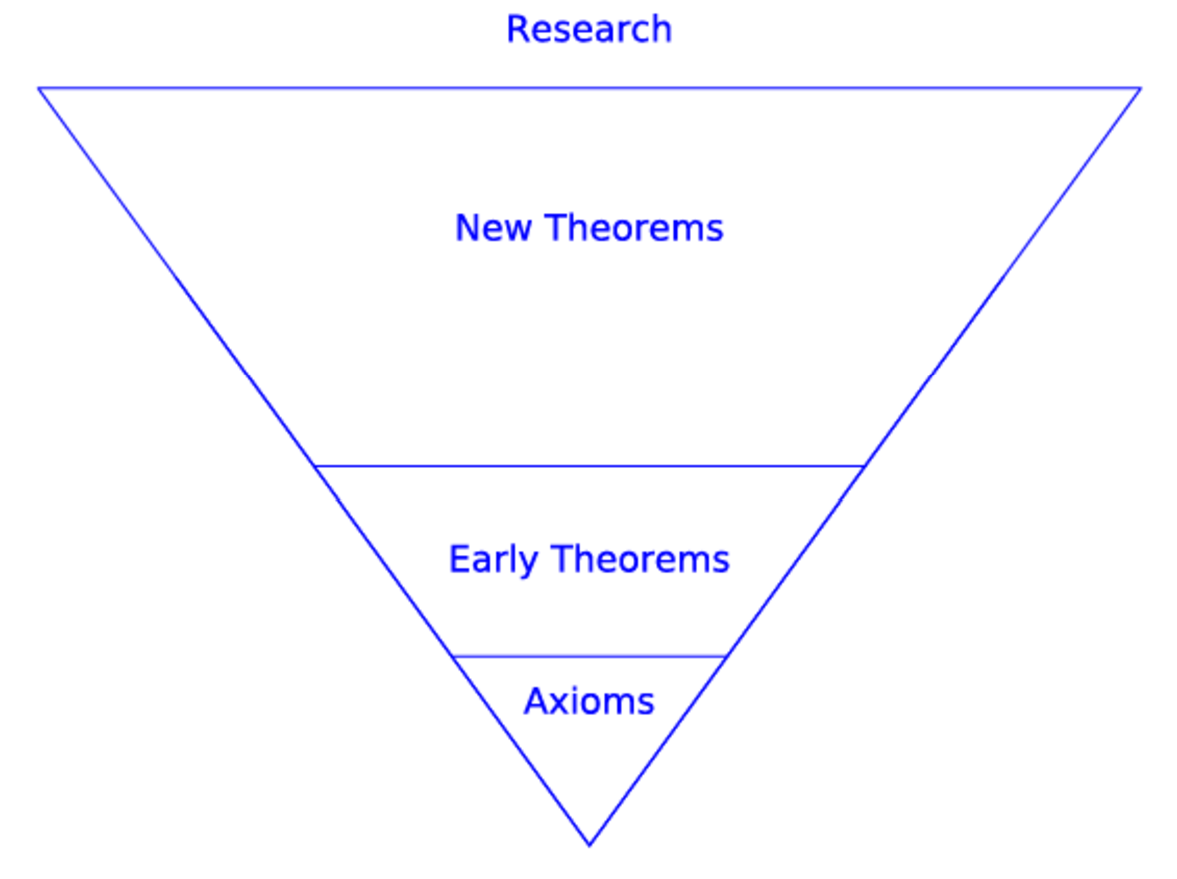
\includegraphics[width=1\linewidth]{images/pyramid.pdf}}%
{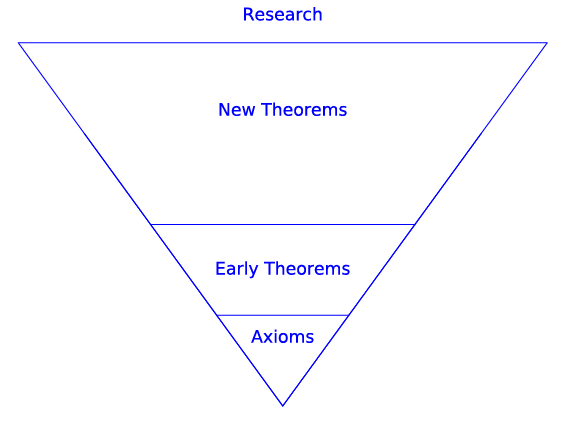
\includegraphics[width=1\linewidth]{images/pyramid.png}}
\caption{The body of knowledge in a mathematical system \label{knowledge-pyramid}}
\end{figure}
\begin{definition}[Proof]\label{def-proof}
 A proof of a theorem is a finite sequence of logically valid steps that demonstrate that the premises of a theorem imply its conclusion.%
\end{definition}
\par
Exactly what constitutes a proof is not always clear. For example, a research mathematician might require only a few steps to prove a theorem to a colleague, but might take an hour to give an effective proof to a class of students. Therefore, what constitutes a proof often depends on the audience. But the audience is not the only factor. One of the most famous theorems in graph theory, The Four Color Theorem, was proven in 1976, after over a century of effort by many mathematicians.  Part of the proof consisted of having a computer check many different graphs for a certain property. Without the aid of the computer, this checking would have taken years. In the eyes of some mathematicians, this proof was considered questionable. Shorter proofs have been developed since 1976 and there is no controversy associated with The Four Color Theorem at this time. (The
theorem is stated in Chapter 9.)%
\par
Theoretically, you can prove anything in propositional calculus with truth tables. In fact, the laws of logic stated in Section 5.4 are all theorems.  Propositional calculus is one of the few mathematical systems for which any valid sentence can be determined true or false by mechanical means. A program to write truth tables is not too difficult to write; however, what can be done theoretically is not always practical. For example,
\begin{equation*}a, a\to  b, b\to  c, . . . ,y\to z\Rightarrow z\end{equation*}
is a theorem in propositional calculus. However, suppose that you wrote such a program and you had it write the truth table for
\begin{equation*}(a\land  (a\to  b)\land ( b\to  c)\land \cdots \land (y\to z))\to z\end{equation*}
The truth table will have \(2^{26}\) cases. At one million cases per second, it would take approximately one hour to verify the theorem.  Now if you decided to check a similar theorem,
\begin{equation*}p_1,p_1\to p_2,\ldots  ,p_{99}\to p_{100}\Rightarrow p_{100}\end{equation*}
you would really have time trouble. There would be \(2^{100} \approx 1.26765\times 10^{30}\) cases to check in the truth table.  At one million cases per second it would take approximately \(1.46719\times 10^{19}\) days to check all cases.  For most of the remainder of this section, we will discuss an alternate method for proving theorems in propositional calculus. It is the same method that we will use in a less formal way for proofs in other systems. Formal axiomatic methods would be too unwieldy to actually use in later sections. However, none of the theorems in later chapters would be stated if they couldn't be proven by the axiomatic method.%
\par
We will introduce two types of proof here, direct and indirect.%
\par
A \terminology{direct proof}\index{Direct proof}%
\begin{example}[A typical direct proof]\label{proof-3-5-1}
 This is a theorem: \(p \rightarrow  r, q\rightarrow s,p\lor q\Rightarrow s\lor r\).   A direct proof of this theorem is:%
\leavevmode%
\begin{table}
\centering
\begin{tabular}{ccc}
Step&Proposition & Justification\tabularnewline[0pt]
1.&\(p \lor  q\)& Premise\tabularnewline[0pt]
2.&\(\neg p \rightarrow  q\)&  (1), conditional rule\tabularnewline[0pt]
3.&\(q \rightarrow  s\)& Premise\tabularnewline[0pt]
4.&\(\neg p \rightarrow  s\)&  (2), (3), chain rule\tabularnewline[0pt]
5.&\(\neg s \rightarrow p\)&  (4), contrapositive\tabularnewline[0pt]
6.&\(p \rightarrow  r\)&  Premise\tabularnewline[0pt]
7.&\(\neg s \rightarrow  r\)& (5), (6), chain rule\tabularnewline[0pt]
8.&\(s \lor r\)& (7), conditional rule   \(\square\)
\end{tabular}
\caption{Direct proof of \(p \rightarrow  r, q\rightarrow s,p\lor q\Rightarrow s\lor r\)\label{proof-steps-1}}
\end{table}
\end{example}
\par
Note that \(\square\) marks the end of a proof.%
\par
Example \hyperref[proof-3-5-1]{\ref{proof-3-5-1}} illustrates the usual method of formal proof in a formal mathematical system. The rules governing these proofs are:%
\par
\leavevmode%
\begin{enumerate}[label=\arabic*]
\item\hypertarget{li-109}{}A proof must end in a finite number of steps.%
\item\hypertarget{li-110}{}Each step must be either a premise or a proposition that is implied from previous steps using any valid equivalence or implication.%
\item\hypertarget{li-111}{}For a direct proof , the last step must be the conclusion of the theorem. For an indirect proof (see below), the last step must be a contradiction.%
\item\hypertarget{li-112}{} Justification Column. The column labeled ``justification'' is analogous to the comments that appear in most good computer programs. They simply make the proof more readable.%
\end{enumerate}
%
\begin{example}[Two proofs of the same theorem]\label{proof-3-5-2}
 Here are two direct proofs of \(\neg p \lor  q, s\lor  p, \neg q \Rightarrow  s\):%
\leavevmode%
\begin{table}
\centering
\begin{tabular}{ccc}
1.&\(\neg p \lor  q\)&Premise\tabularnewline[0pt]
2.&\(\neg q\)&Premise\tabularnewline[0pt]
3.&\(\neg p\)&Disjunctive simplification, (1), (2)\tabularnewline[0pt]
4.&\(s\lor  p\)&Premise\tabularnewline[0pt]
5.&\(s\)&Disjunctive simplification, (3), (4). \(\square\)
\end{tabular}
\caption{Direct proof of  \(\neg p \lor  q, s\lor  p, \neg q \Rightarrow  s\)\label{proof-steps-2}}
\end{table}
\par
You are invited to justify the steps in this second proof:%
\leavevmode%
\begin{table}
\centering
\begin{tabular}{cc}
1.&\(\neg p \lor  q\)\tabularnewline[0pt]
2.&\(\neg q \rightarrow  \neg p\)\tabularnewline[0pt]
3.&\(s\lor p\)\tabularnewline[0pt]
4.&\(p \lor  s\)\tabularnewline[0pt]
5.&\(\neg p \to s\)\tabularnewline[0pt]
6.&\(\neg q \rightarrow  s\)\tabularnewline[0pt]
7.&\(\neg q\)\tabularnewline[0pt]
8.&\(s\)    \(\square\)
\end{tabular}
\caption{Alternate  proof of  \(\neg p \lor  q, s\lor  p, \neg q \Rightarrow  s\)\label{proof-steps-2a}}
\end{table}
\end{example}
\par
The conclusion of a theorem is often a conditional proposition. The condition of the conclusion can be included as a premise in the proof of the theorem. The object of the proof is then to prove the consequence of the conclusion. This rule is justified by the logical law
\begin{equation*}p \rightarrow  (h \rightarrow  c) \Leftrightarrow  (p \land  h) \rightarrow  c\end{equation*}
%
\begin{example}[Example of a proof with a conditional conclusion]\label{ex-conditinal-conclusion}
The following proof of \(p \to  (q \rightarrow  s), \neg r  \lor p, q \Rightarrow r \rightarrow s\) includes
\(r\) as a fourth premise. Inference of truth of \(s\) completes the proof.%
\leavevmode%
\begin{table}
\centering
\begin{tabular}{ccc}
1.&\(\neg r \lor p\)&  Premise\tabularnewline[0pt]
2.&\(r\)&  Added premise\tabularnewline[0pt]
3.&\(p\)&  (1), (2), disjunction simplification\tabularnewline[0pt]
4.&\(p \rightarrow  (q \to s)\)& Premise\tabularnewline[0pt]
5.&\(q\rightarrow s\)&  (3), (4), detachment\tabularnewline[0pt]
6.&\(q\)&  Premise\tabularnewline[0pt]
7.&\(s\)&   (5), (6), detachment. \(\square\) 
\end{tabular}
\caption{Proof of a theorem with a conditional conclusion.\label{proof-conditional-conclusion}}
\end{table}
\end{example}
\par
Consider a theorem \(P\Rightarrow C\), where \(P\) represents \(p_1, p_2, . . . , \textrm{ and } p_n\), the premises. The method of \terminology{indirect proof}\index{Indirect proof} is based on the equivalence \(P\rightarrow C\Leftrightarrow \neg (P\land  \neg C)\). 
In words, this logical law states that if \(P \Rightarrow  C\), then \(P \land  \neg  C\) is always false; that is, \(P \land  \neg C\) is a contradiction. This means that a valid method of proof is to negate the conclusion of a theorem and add this negation to the premises. If a contradiction can be implied from this set of propositions, the proof is complete. For the proofs in this section, a contradiction will often take the form \(t \land \neg t\).%
\par
 For proofs involving numbers, a contradiction might be \(1 = 0\) or \(0 < 0\). Indirect proofs involving sets might conclude with \(x \in  \emptyset\) or (\(x \in  A\) and \(x \in  A^c\)). Indirect proofs are often more convenient than direct proofs in certain situations.  Indirect proofs are often called \emph{proofs by contradiction}.%
\begin{example}[An Indirect Proof]\label{ex-indirect_proof_1}
 Here is an example of an indirect proof of the theorem in \hyperref[proof-3-5-1]{Example~\ref{proof-3-5-1}}.%
\leavevmode%
\begin{table}
\centering
\begin{tabular}{ccc}
1.&\(\neg (s \lor  r)\)&  Negated conclusion\tabularnewline[0pt]
2.&\(\neg s \land  \neg r\)&  DeMorgan's Law, (1)\tabularnewline[0pt]
3.&\(\neg s\)& Conjunctive simplification, (2)\tabularnewline[0pt]
4.&\(q\to s\)&  Premise\tabularnewline[0pt]
5.&\(\neg q\)&  Indirect reasoning, (3), (4)\tabularnewline[0pt]
6.&\(\neg r\)&  Conjunctive simplification, (2)\tabularnewline[0pt]
7.&\(p \rightarrow  r\)& Premise\tabularnewline[0pt]
8.&\(\neg p\)&  Indirect reasoning, (6), (7)\tabularnewline[0pt]
9.&\((\neg p) \land  (\neg q)\)&  Conjunctive, (5), (8)\tabularnewline[0pt]
10.&\(\neg (p \lor  q)\)&DeMorgan's Law, (9)\tabularnewline[0pt]
11.&\(p \lor  q\)&Premise\tabularnewline[0pt]
12.&\(0\)&(10), (11) \(\square\)
\end{tabular}
\caption{An Indirect proof of \(p \rightarrow  r, q\rightarrow s,p\lor q\Rightarrow s\lor r\)\label{proof-indirect}}
\end{table}
\end{example}
\begin{note}[Proof Style]\label{note-1}
The rules allow you to list the premises of a theorem immediately; however, a proof is much easier to follow if the premises are only listed when they are needed.%
\end{note}
\begin{example}[Yet Another Indirect Proof]\label{proof-yet-another}
 Here is an indirect proof of \(a \rightarrow  b, \neg (b \lor  c ) \Rightarrow  \neg  a\).%
\leavevmode%
\begin{table}
\centering
\begin{tabular}{ccc}
1.&\(a\)&  Negation of the conclusion\tabularnewline[0pt]
2.&\(a\to  b\)&Premise\tabularnewline[0pt]
3.&\(b\)&  (1), (2), detachment\tabularnewline[0pt]
4.&\(b \lor  c\)&  (3), disjunctive addition\tabularnewline[0pt]
5.&\(\neg (b \lor  c)\)&  Premise\tabularnewline[0pt]
6.&\(0\)&  (4), (5)  \(\square\)
\end{tabular}
\caption{Indirect proof of \(a \rightarrow  b, \neg (b \lor  c ) \Rightarrow  \neg  a\)\label{proof-style}}
\end{table}
\end{example}
\par
As we mentioned at the outset of this section, we are only presenting an overview of what a mathematical system is. For greater detail on axiomatic theories, see Stoll (1961). An excellent description of how propositional calculus plays a part in artificial intelligence is contained in Hofstadter (1980). If you enjoy the challenge of constructing proofs in propositional calculus, you should enjoy the game WFF'N PROOF (1962), by L.E. Allen.%
\typeout{************************************************}
\typeout{Exercises 1.5.1 Exercises for Section 3.5 }
\typeout{************************************************}
\subsection[Exercises for Section 3.5 ]{Exercises for Section 3.5 }\label{exercises-3.5}
\hypertarget{exercisegroup-6}{}\typeout{************************************************}
\typeout{Introduction  }
\typeout{************************************************}
A Exercises%
\begin{exercisegroup}
\item[1.]\hypertarget{exercise-24}{} Prove with truth tables:%
\par
\leavevmode%
\begin{enumerate}[label=\alph*]
\item\hypertarget{li-113}{} \(p\lor  q, \neg q\Rightarrow  p\)%
\item\hypertarget{li-114}{} \(p \rightarrow  q, \neg q \Rightarrow  \neg p\)%
\end{enumerate}

%
\par\smallskip
\par\smallskip
\noindent\textbf{Answer.}\hypertarget{answer-11}{}\quad
\leavevmode%
\begin{enumerate}[label=\alph*]
\item\hypertarget{li-115}{}  
\[
 \begin{array}{cccc}
 p & q &  (p\lor q)\land \neg q & ((p\lor q)\land \neg q)\to p \\
 0 & 0 & 0 & 1 \\
 0 & 1 & 0 & 1 \\
 1 & 0 & 1 & 1 \\
 1 & 1 & 0 & 1 \\
\end{array}
\] %
\item\hypertarget{li-116}{} \[\begin{array}{ccccc}
 p & q  & (p\to q)\land \neg q & \neg p & (p\to q)\land (\neg q) \\
 0 & 0 & 1 & 1 & 1 \\
 0 & 1 & 0 & 1 & 1 \\
 1 & 0 & 0 & 0 & 1 \\
 1 & 1 & 0 & 0 & 1 \\
\end{array}\]%
\end{enumerate}
%
\item[2.]\hypertarget{exercise-25}{} Prove with truth tables:%
\par
\leavevmode%
\begin{enumerate}[label=\alph*]
\item\hypertarget{li-117}{} \(q, \neg q\Rightarrow  p\)%
\item\hypertarget{li-118}{}  \(p \rightarrow  q \Rightarrow  \neg p \lor  q\)%
\end{enumerate}

%
\par\smallskip
\end{exercisegroup}
\par\smallskip\noindent
\hypertarget{exercisegroup-7}{}\typeout{************************************************}
\typeout{Introduction  }
\typeout{************************************************}
B Exercises%
\begin{exercisegroup}
\item[3.]\hypertarget{exercise-26}{}Give direct and indirect proofs of:%
\par
\leavevmode%
\begin{enumerate}[label=\alph*]
\item\hypertarget{li-119}{}\(a \rightarrow  b, c \rightarrow  b, d\rightarrow  (a \lor  c), d\Rightarrow  b\).%
\item\hypertarget{li-120}{} \((p\to q) \land (r\to s), (q\rightarrow t) \land  (s \to  u), \neg (t \land u), p \rightarrow  r \Rightarrow  \neg p\).%
\item\hypertarget{li-121}{}\(p\to (q\to r),\neg s\text{$\backslash $/}p,q\Rightarrow s\to r\).%
\item\hypertarget{li-122}{} \(p\rightarrow  q, q\rightarrow  r, \neg (p \land  r), p \lor  r \Rightarrow  r\).%
\item\hypertarget{li-123}{}\(\neg q, p\to q, p\lor t \Rightarrow t\)%
\end{enumerate}
%
\par\smallskip
\par\smallskip
\noindent\textbf{Answer.}\hypertarget{answer-12}{}\quad
\leavevmode%
\begin{enumerate}[label=\alph*]
\item\hypertarget{li-124}{}%
\begin{enumerate}[label=\arabic*]
\item\hypertarget{li-125}{} Direct proof:%
\item\hypertarget{li-126}{} \(d\to (a\lor c)\)%
\item\hypertarget{li-127}{} \(d\)%
\item\hypertarget{li-128}{} \(a\lor c\)%
\item\hypertarget{li-129}{} \(a\to b\)%
\item\hypertarget{li-130}{} \(\neg a \lor b\)%
\item\hypertarget{li-131}{} \(c\to b\)%
\item\hypertarget{li-132}{} \(\neg c\lor b\)%
\item\hypertarget{li-133}{} \((\neg a\lor b)\land (\neg c\lor b)\)%
\item\hypertarget{li-134}{} \((\neg a\land \neg c) \lor b\)%
\item\hypertarget{li-135}{} \(\neg (a\lor c)\lor b\)%
\item\hypertarget{li-136}{} \(b\) \(\square\)%
\end{enumerate}
%
\par
Indirect proof:%
\par
%
\begin{enumerate}[label=\arabic*]
\item\hypertarget{li-137}{} \(\neg b\quad \)   Negated conclusion%
\item\hypertarget{li-138}{} \(a\to b\quad \)    Premise%
\item\hypertarget{li-139}{} \(\neg a\quad \)   Indirect Reasoning (1), (2)%
\item\hypertarget{li-140}{} \(c\to b\quad \)   Premise%
\item\hypertarget{li-141}{} \(\neg c\quad \)     Indirect Reasoning (1), (4)%
\item\hypertarget{li-142}{} \((\neg a\land \neg c)\quad \)     Conjunctive (3), (5)%
\item\hypertarget{li-143}{} \(\neg (a\lor c)\quad \)   DeMorgan's law (6)%
\item\hypertarget{li-144}{} \(d\to (a\lor c)\quad \)    Premise%
\item\hypertarget{li-145}{} \(\neg d\quad \)    Indirect Reasoning (7), (8)%
\item\hypertarget{li-146}{} \(d\quad \)  Premise%
\item\hypertarget{li-147}{} \(\mathbb{0} \quad \)  (9), (10) \(\quad \square\)%
\end{enumerate}
%
\item\hypertarget{li-148}{}Direct proof:%
\par
%
\begin{enumerate}[label=\arabic*]
\item\hypertarget{li-149}{} \((p\to q)\land (r\to s)\)%
\item\hypertarget{li-150}{} \(p\to q\)%
\item\hypertarget{li-151}{} \((p\to t)\land (s\to u)\)%
\item\hypertarget{li-152}{} \(q\to t\)%
\item\hypertarget{li-153}{} \(p\to t\)%
\item\hypertarget{li-154}{} \(r\to s\)%
\item\hypertarget{li-155}{} \(s\to u\)%
\item\hypertarget{li-156}{} \(r\to u\)%
\item\hypertarget{li-157}{} \(p\to r\)%
\item\hypertarget{li-158}{}\(p\to u\)%
\item\hypertarget{li-159}{}\(p\to (t\land u)\) Use \((x\to y)\land (x\to z)\Leftrightarrow x\to (y\land z)\)%
\item\hypertarget{li-160}{} \(\neg (t\land u)\to \neg p\)%
\item\hypertarget{li-161}{} \(\neg (t\land u)\)%
\item\hypertarget{li-162}{}\(\neg p\) \(\quad \square\)%
\end{enumerate}
%
\par
Indirect proof:%
\par
%
\begin{enumerate}[label=\arabic*]
\item\hypertarget{li-163}{}  \(p\)%
\item\hypertarget{li-164}{} \(p\to q\)%
\item\hypertarget{li-165}{} \(q\)%
\item\hypertarget{li-166}{}\(q\to t\)%
\item\hypertarget{li-167}{} \(t\)%
\item\hypertarget{li-168}{} \(\neg (t\land u)\)%
\item\hypertarget{li-169}{}\(\neg t\lor \neg u\)%
\item\hypertarget{li-170}{} \(\neg u\)%
\item\hypertarget{li-171}{} \(s\to u\)%
\item\hypertarget{li-172}{} \(\neg s\)%
\item\hypertarget{li-173}{}\(r\to s\)%
\item\hypertarget{li-174}{} \(\neg r\)%
\item\hypertarget{li-175}{} \(p\to r\)%
\item\hypertarget{li-176}{}\(r\)%
\item\hypertarget{li-177}{} \(0\) \(\quad \square\)%
\end{enumerate}
%
\item\hypertarget{li-178}{} Direct proof:%
\par
%
\begin{enumerate}[label=\arabic*]
\item\hypertarget{li-179}{} \(\neg s\lor p\quad \)   Premise%
\item\hypertarget{li-180}{} \(s\quad \)    Added premise (conditional conclusion)%
\item\hypertarget{li-181}{} \(\neg (\neg s)\quad \)   Involution (2)%
\item\hypertarget{li-182}{} \(p\)  \quad  Disjunctive simplification (1), (3)%
\item\hypertarget{li-183}{} \(p\to (q\to r)\quad \)    Premise%
\item\hypertarget{li-184}{} \(q\to r\quad \)    Detachment (4), (5)%
\item\hypertarget{li-185}{} \(q\)  Premise%
\item\hypertarget{li-186}{} \(r\quad \)     Detachment (6), (7) \(\square\) %
\end{enumerate}
%
\par
Indirect proof:%
\par
%
\begin{enumerate}[label=\arabic*]
\item\hypertarget{li-187}{} \(\neg (s\to r)\quad \)    Negated conclusion%
\item\hypertarget{li-188}{} \(\neg (\neg s\lor r)\quad \)  Conditional equivalence (I)%
\item\hypertarget{li-189}{} \(s\land \neg r\quad \)   DeMorgan (2)%
\item\hypertarget{li-190}{} \(s\quad\) Conjunctive simplification (3)%
\item\hypertarget{li-191}{} \(\neg s\lor p\quad \)   Premise%
\item\hypertarget{li-192}{} \(s\to p\quad\)   Conditional equivalence (5)%
\item\hypertarget{li-193}{} \( p  \quad\)  Detachment (4), (6)%
\item\hypertarget{li-194}{} \(p\to (q\to r)\quad\)   Premise%
\item\hypertarget{li-195}{} \(q\to r \quad\)  Detachment (7), (8)%
\item\hypertarget{li-196}{} \(q\quad \)   Premise%
\item\hypertarget{li-197}{} \(r\quad\)   Detachment (9), (10)%
\item\hypertarget{li-198}{} \(\neg r \quad\) Conjunctive simplification (3)%
\item\hypertarget{li-199}{} \(0\)  \quad Conjunction (11), (12) \(\square\)%
\end{enumerate}
%
\item\hypertarget{li-200}{} Direct proof:%
\par
%
\begin{enumerate}[label=\arabic*]
\item\hypertarget{li-201}{} \(p\to q\)%
\item\hypertarget{li-202}{} \(q\to r\)%
\item\hypertarget{li-203}{} \(p\to r\)%
\item\hypertarget{li-204}{} \(p\lor r\)%
\item\hypertarget{li-205}{} \(\neg p\lor r\)%
\item\hypertarget{li-206}{} \((p\lor r)\land (\neg p\lor r)\)%
\item\hypertarget{li-207}{} \((p\land \neg p)\lor r\)%
\item\hypertarget{li-208}{} \(0\lor r\)%
\item\hypertarget{li-209}{} \(r\)\(\square\)%
\end{enumerate}
%
\par
Indirect proof:%
\par
%
\begin{enumerate}[label=\arabic*]
\item\hypertarget{li-210}{} \(\neg r\) Negated conclusion%
\item\hypertarget{li-211}{} \(p\lor r\) Premise%
\item\hypertarget{li-212}{}  \(p\)   (1), (2)%
\item\hypertarget{li-213}{} \(p\to q\) Premise%
\item\hypertarget{li-214}{} \(q \quad \)  Detachment (3), (4)%
\item\hypertarget{li-215}{} \(q\to r\)  Premise%
\item\hypertarget{li-216}{} \(r \quad \)Detachment (5), (6)%
\item\hypertarget{li-217}{} 0   (1), (7) \(\square\)%
\end{enumerate}
%
\end{enumerate}
%
\item[4.]\hypertarget{exercise-27}{}Give direct and indirect proofs of:%
\par
\leavevmode%
\begin{enumerate}[label=\alph*]
\item\hypertarget{li-218}{} \(p\rightarrow  q, \neg r\rightarrow  \neg q, \neg r \Rightarrow  \neg p\).%
\item\hypertarget{li-219}{} \(p\rightarrow  \neg q, \neg r\rightarrow  q, p \Rightarrow  r\).%
\item\hypertarget{li-220}{} \(a \lor  b, c \land  d, a \rightarrow  \neg c \Rightarrow  b\).%
\end{enumerate}
%
\par\smallskip
\item[5.]\hypertarget{exercise-28}{}Are the following arguments valid? If they are valid, construct formal proofs; if they aren't valid, explain why not.%
\par
\leavevmode%
\begin{enumerate}[label=\alph*]
\item\hypertarget{li-221}{}If wages increase, then there will be inflation. The cost of living will not increase if there is no inflation. Wages will increase. Therefore, the cost of living will increase.%
\item\hypertarget{li-222}{}If the races are fixed or the casinos are crooked, then the tourist trade will decline. If the tourist trade decreases, then the police will be happy. The police force is never happy. Therefore, the races are not fixed.%
\end{enumerate}
%
\par\smallskip
\par\smallskip
\noindent\textbf{Answer.}\hypertarget{answer-13}{}\quad
\leavevmode%
\begin{enumerate}[label=\alph*]
\item\hypertarget{li-223}{} Let \(W\) stand for ``Wages will increase,''\(I\)
 stand for ``there will be inflation,'' and \(C\) stand for ``cost of living will increase.'' Therefore the argument is: \(W\to I,\text{   }\neg I\to \neg C,\text{   }W\Rightarrow C.\). The argument is invalid. The easiest way to see this is through a truth table. Let \(x\) be the conjunction of all premises.

 \(\begin{array}{ccccccccc}
 W  & I  & C  & \neg I  & \neg C  & W\to I  & \neg I\to \neg C  & x  & x\to C \\
\hline
 0  & 0  & 0  & 1  & 1 & 1  & 0  & 0  & 1 \\
 0  & 0  & 1  & 1  & 0 & 1  & 1  & 0  & 1 \\
 0  & 1  & 0  & 0  & 1 & 1  & 1  & 0  & 1 \\
 0  & 1  & 1  & 0  & 0 & 1  & 1  & 0  & 1 \\
 1  & 0  & 0  & 1  & 1 & 0  & 0  & 0  & 1 \\
 1  & 0  & 1  & 1  & 0 & 0  & 1  & 0  & 1 \\
 1  & 1  & 0  & 0  & 1 & 1  & 1  & 1  & 1 \\
 1  & 1  & 1  & 0  & 0 & 1  & 1  & 1  & 0 \\
\end{array}\)%
\item\hypertarget{li-224}{}Let \(r\) stand for ``the races are fixed,'' \(c\) stand for ``casinos are crooked,'' \(t\) stand for ``the tourist trade will decline,'' and \(p\) stand for ``the police will be happy.'' Therefore, the argument is:

\[(r\lor c)\to t, t\to p, \neg p\to \neg r\]. The argument is valid. Proof:%
\par
%
\begin{enumerate}[label=\arabic*]
\item\hypertarget{li-225}{} \(t\to p\quad \)   Premise%
\item\hypertarget{li-226}{} \(\neg p\quad \)   Premise%
\item\hypertarget{li-227}{} \(\neg t\quad \)   Indirect Reasoning (1), (2)%
\item\hypertarget{li-228}{} \((r\lor c)\to t\quad \)     Premise%
\item\hypertarget{li-229}{} \(\neg (r\lor c)\quad \)   Indirect Reasoning (3), (4)%
\item\hypertarget{li-230}{} \((\neg r)\land (\neg c)\quad \)   DeMorgan (5)%
\item\hypertarget{li-231}{} \(\neg r\quad \)     Conjunction simplification \((6)\text{    }\square\)%
\end{enumerate}
%
\end{enumerate}
%
\item[6.]\hypertarget{exercise-29}{}Determine the validity of the following argument: For students to do well in a discrete mathematics course, it is necessary that they study hard.
Students who do well in courses do not skip classes. Students who study hard do well in courses. Therefore students who do well in a discrete mathematics
course do not skip class.%
\par\smallskip
\item[7.]\hypertarget{exercise-30}{}Describe how \(p_1,p_1\to p_2,\ldots  ,p_{99}\to p_{100}\Rightarrow p_{100}\) could be proven in 199 steps.
%
\par\smallskip
\par\smallskip
\noindent\textbf{Answer.}\hypertarget{answer-14}{}\quad
 \(p_1\to p_k\) and \(p_k\to p_{k+1}\) implies \(p_1\to p_{k+1}\). It takes two steps to get to \(p_1\to p_{k+1}\) from \(p_1\to p_k\) This means it takes \(2(100-1)\) steps to get to \(p_1\to p_{100}\) (subtract 1 because \(p_1\to p_2\) is stated as a premise). A final step is needed to apply detachment to imply \(p_{100}\)%
\end{exercisegroup}
\par\smallskip\noindent
\typeout{************************************************}
\typeout{Section 1.6 Propositions over a Universe}
\typeout{************************************************}
\section[Propositions over a Universe]{Propositions over a Universe}\label{c3s6}
\typeout{************************************************}
\typeout{Subsection 1.6.1 Propositions over a Universe}
\typeout{************************************************}
\subsection[Propositions over a Universe]{Propositions over a Universe}\label{ss-propositions-over-a-universe}
Consider the sentence ``He was a member of the Boston Red Sox.'' There is no way that we can assign a truth value to this sentence unless ``he'' is specified. For that reason, we would not consider it a proposition. However, ``he'' can be considered a variable that holds a place for any name. We might want to restrict the value of ``he'' to all names in the major-league baseball record books. If that is the case, we say that the sentence is a proposition over the set of major-league baseball players, past and present.%
\begin{definition}[Proposition over a Universe]\label{def-proposition-over-U}
Let \(U\) be a nonempty set. A proposition over \(U\) is a sentence that contains a variable that can take on any value in \(U\) and that has a definite truth value as a result of any such substitution.%
\end{definition}
\begin{example}[Some propositions over a variety of universes]\label{ex-some-propositions-over-U}

	\leavevmode%
\begin{enumerate}
\item\hypertarget{li-232}{} A few propositions over the integers are \(4x^2 - 3x = 0\),  \(0 \leq  n \leq 5\), and ``\(k\) is a multiple of 3.''%
\item\hypertarget{li-233}{} A few propositions over the rational numbers are \(4x^2 - 3x = 0\),  \(y^2=2\), and  \((s - 1)(s + 1) = s^2 - 1\).%
\item\hypertarget{li-234}{} A few propositions over the subsets of \(\mathbb{P}\) are \((A =\emptyset ) \lor  (A = \mathbb{P} )\), \(3 \in  A\), and  \(A \cap  \{1, 2, 3\}\neq  \emptyset\).%
\end{enumerate}

	%
\end{example}
\par
All of the laws of logic that we listed in Section 3.4 are valid for propositions over a universe. For example, if \(p\) and \(q\) are propositions over the integers, we can be certain that \(p \land  q \Rightarrow  p\), because \((p \land  q) \to  p\) is a tautology and is true no matter what values the variables in \(p\) and \(q\) are given. If we specify \(p\) and \(q\) to be \(p(n) : n < 4\) and \(q(n) : n < 8\), we can also say that \(p\) implies \(p \land  q\). This is not a usual implication, but for the propositions under discussion, it is true. One way of describing this situation in general is with truth sets.%
\typeout{************************************************}
\typeout{Subsection 1.6.2 Truth Sets}
\typeout{************************************************}
\subsection[Truth Sets]{Truth Sets}\label{ss-truth-sets}
\begin{definition}[Truth Set]\label{def-truth-set}
\index{Truth Set}\label{notation-11}
If \(p\) is a proposition over \(U\), the truth set of \(p\) is \(T_p = \{a \in  U \mid p(a) \textrm{ is true}\}\).%
\end{definition}
\begin{example}[Truth Set Example]\label{ex-set-prop}
The truth set of the proposition \(\{1, 2\} \cap A = \emptyset\), taken as a proposition over the power set of \(\{1, 2, 3, 4\}\) is \(\{\emptyset , \{3\}, \{4\}, \{3, 4\}\}\).
%
\end{example}
\begin{example}[Truth sets depend on the universe]\label{ex-vary-U}
Over the universe \(mathbb{Z}\) (the integers), the truth set of \(4x^2- 3x = 0\) is \(\{0\}\). If the universe is expanded to the rational numbers, the truth set becomes \(\{0, 3/4\}\). The term \emph{solution set} is often used for the truth set of an equation such as the one in this example.%
\end{example}
\begin{definition}[Tautologys and Contradictions over a Universe]\label{def-tautology-contradiction-over-U}
 A proposition over \(U\) is a tautology if its truth set is \(U\). It is a contradiction if its truth set is empty.%
\end{definition}
\begin{example}[Tautology, Contradiction over \(\mathbb{Q}\)]\label{ex-tautology-contradiction-over-U}
 \((s - 1)(s + 1) = s^2 - 1\) is a tautology over the rational numbers. \(x^2-2 = 0\) is a contradiction over the rationals.%
\end{example}
The truth sets of compound propositions can be expressed in terms of the truth sets of simple propositions. For example, if \(a \in  T_{p\land q}\) if and only if \(a\) makes \(p \land  q\) true. This is true iff an only if  \(a\) makes both \(p\) and \(q\) true, which which, in turn, is true if and only if  \(a \in  T_p\cap T_q\). This explains why the truth set of the conjunction of two propositions equals the intersection of the truth sets of the two propositions. The following list summarizes the connection between compound and simple truth sets%
\leavevmode%
\begin{table}
\centering
\begin{tabular}{c}
\(T_{p\land q}=T_p\cap T_q\)\tabularnewline[0pt]
\(T_{p\lor q}=T_p\cup T_q\)\tabularnewline[0pt]
\(T_{\neg p}=T_p{}^c\)\tabularnewline[0pt]
\(T_{p\leftrightarrow q}=\left(T_p\cap T_q\right)\cup \left(T_p{}^c\cap T_q{}^c\right)\)\tabularnewline[0pt]
\(T_{p\to q}=T_p{}^c\cup T_q\)
\end{tabular}
\caption{Truth Sets of Compound Statements\label{table-truth-sets-compound-statements}}
\end{table}
\begin{definition}[Equivalence of propositions over a universe]\label{def-equivanlence-over-U}
Two propositions are equivalent if \(p \leftrightarrow  q\) is a tautology. In terms of truth sets, this means that \(p\) and \(q\) are equivalent if \(T_p=T_q\) .
%
\end{definition}
\begin{example}[Some pairs of equivalent propositions.]\label{ex-some-equivalent-pairs}
\leavevmode%
\begin{enumerate}[label=\alph*]
\item\hypertarget{li-235}{}  \(n + 4 = 9\) and \(n = 5\) are equivalent propositions over the integers.%
\item\hypertarget{li-236}{} \(A \cap  \{4\} \neq  \emptyset\) and \(4 \in  A\) are equivalent propositions over the power set of the natural numbers.%
\end{enumerate}

%
\end{example}
\begin{definition}[Implication for propositions over a universe]\label{def-implication-over-U}
 Implication. If \(p\) and \(q\) are propositions over U, \(p\) implies \(q\) if \(p \rightarrow >q\) is a tautology.%
\end{definition}
\par
Since the truth set of \(p \rightarrow  q\) is \(T_p{}^c\cup T_q\), the Venn diagram for \(T_{p\to q}\) in Figure 3.6.1 shows that \(p \Rightarrow  q\) when \(T_p\subseteq T_q\).%
\leavevmode%
\begin{figure}
\centering
\IfFileExists{images/sageplot-venn-truth-set-conditional.pdf}%
{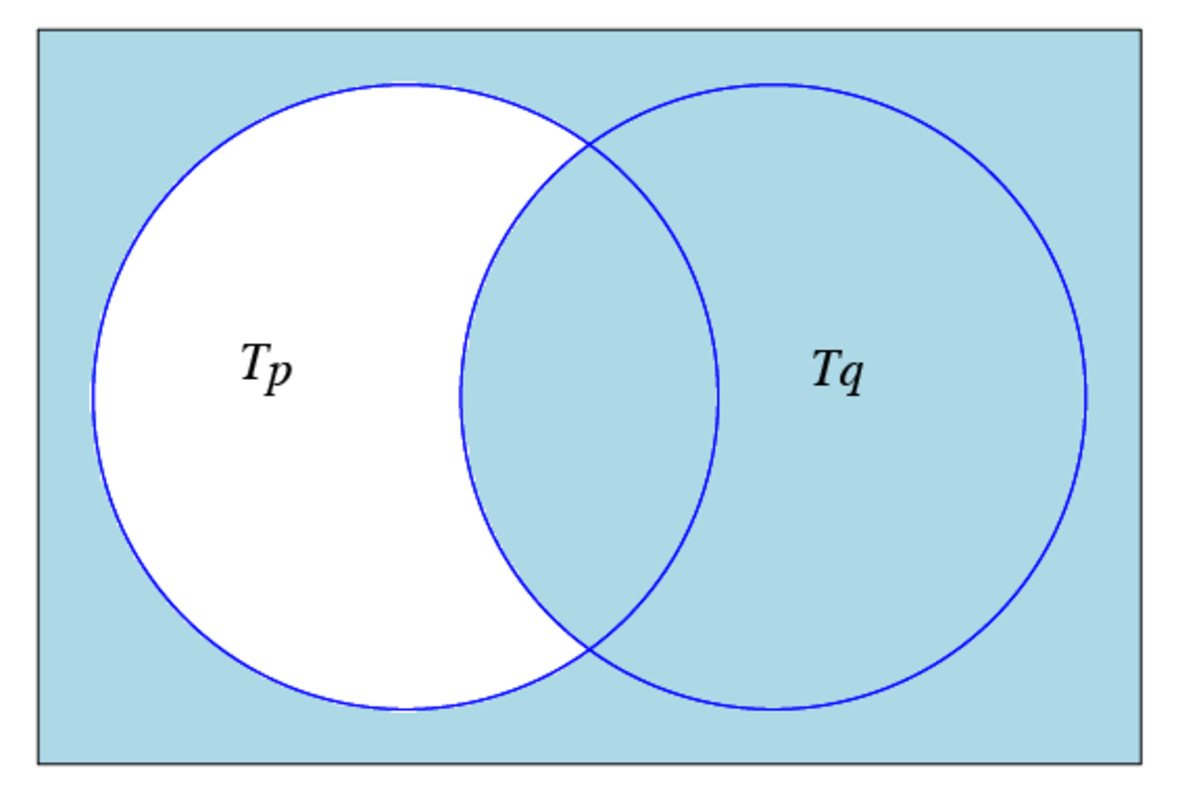
\includegraphics[width=1\linewidth]{images/sageplot-venn-truth-set-conditional.pdf}}%
{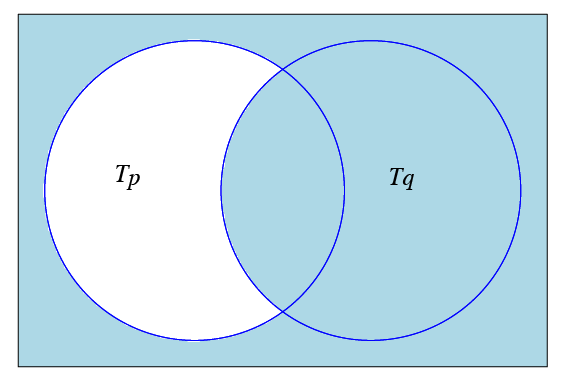
\includegraphics[width=1\linewidth]{images/sageplot-venn-truth-set-conditional.png}}
\caption{Venn Diagram for \(T_{p\to q}\) \label{venn_diagram_truth_set_conditional}}
\end{figure}
\begin{example}[Examples of Implications]\label{ex-implications-over-U}
\leavevmode%
\begin{enumerate}[label=\alph*]
\item\hypertarget{li-237}{} Over the natural numbers: \(n < 4 \Rightarrow  n < 8\) since \(\{0, 1, 2, 3, 4\} \subseteq  \{0, 1, 2, 3, 4, 5, 6, 7, 8\}\)%
\item\hypertarget{li-238}{}  Over the power set of the integers: \(\lvert A^c \rvert=1\) implies \(A\cap \{0,1\}\neq \emptyset\)%
\item\hypertarget{li-239}{} \(A \subseteq  \textrm{ even integers } \Rightarrow  A\cap  \textrm{ odd integers } =\emptyset\)%
\end{enumerate}
%
\end{example}
\typeout{************************************************}
\typeout{Exercises 1.6.3 Exercises for Section 3.6 }
\typeout{************************************************}
\subsection[Exercises for Section 3.6 ]{Exercises for Section 3.6 }\label{exercises-3.6}
\hypertarget{exercisegroup-8}{}\typeout{************************************************}
\typeout{Introduction  }
\typeout{************************************************}
A Exercises%
\begin{exercisegroup}
\item[1.]\hypertarget{exercise-31}{} If \(U = \mathcal{P}( \{1, 2, 3, 4\})\), what are the truth sets of the following propositions?%
\par
\leavevmode%
\begin{enumerate}[label=\alph*]
\item\hypertarget{li-240}{} \(A \cap  \{2, 4\} = \emptyset\).%
\item\hypertarget{li-241}{} \(3 \in  A\) and \(1 \notin  A\).%
\item\hypertarget{li-242}{} \(A \cup  \{1\} = A\).%
\item\hypertarget{li-243}{}  \(A\) is a proper subset of \(\{2, 3, 4\}\).%
\item\hypertarget{li-244}{} \(\lvert A \rvert=\lvert A^c \rvert\).%
\end{enumerate}

%
\par\smallskip
\par\smallskip
\noindent\textbf{Answer.}\hypertarget{answer-15}{}\quad

\leavevmode%
\begin{enumerate}[label=\alph*]
\item\hypertarget{li-245}{} \(\{\{1\},\{3\},\{1,3\},\text{\(\emptyset\)}\}\)%
\item\hypertarget{li-246}{} \(\{\{3\}, \{3,4\}, \{3,2\}, \{2,3,4\}\}\)%
\item\hypertarget{li-247}{} \(\{\{1\}, \{1,2\}, \{1,3\}, \{1,4\}, \{1,2,3\}, \{1,2,4\}, \{1,3,4\}, \{1,2,3,4\}\}\)%
\item\hypertarget{li-248}{} \(\{\{2\}, \{3\}, \{4\}, \{2,3\}, \{2,4\}, \{3,4\}\}\)%
\item\hypertarget{li-249}{} \(\{A\subseteq U:\left| A\right| =2\}\)%
\end{enumerate}
%
\item[2.]\hypertarget{exercise-32}{}Over the universe of positive integers, define%
\leavevmode%
\begin{table}
\centering
\begin{tabular}{ll}
\(p(n)\):& \(n\) is prime and \(n < 32\).\tabularnewline[0pt]
\(q(n)\):& \(n\) is a power of 3.\tabularnewline[0pt]
\(r(n)\):& \(n\) is a divisor of 27.
\end{tabular}
\end{table}
\par
\leavevmode%
\begin{enumerate}[label=\alph*]
\item\hypertarget{li-250}{}  What are the truth sets of these propositions?%
\item\hypertarget{li-251}{}  Which of the three propositions implies one of the others?%
\end{enumerate}
%
\par\smallskip
\par\smallskip
\noindent\textbf{Solution.}\hypertarget{solution-3}{}\quad
\leavevmode%
\begin{enumerate}[label=\alph*]
\item\hypertarget{li-252}{}%
\begin{enumerate}[label=\roman*]
\item\hypertarget{li-253}{} \(T_p = \{2, 3, 5, 7, 11, 13, 17, 19, 23, 29, 31 \}\)%
\item\hypertarget{li-254}{} \(T_q = \{1, 3, 9, 27, 81, \dots \}\)%
\item\hypertarget{li-255}{} \(T_r = \{1, 3, 9, 27 \}\)%
\end{enumerate}
%
\item\hypertarget{li-256}{} \( r \Rightarrow q \) %
\end{enumerate}
%
\item[3.]\hypertarget{exercise-33}{}  If \(U = \{0, 1, 2\}\), how many propositions over \(U\) could you list without listing two that are equivalent?
%
\par\smallskip
\par\smallskip
\noindent\textbf{Answer.}\hypertarget{answer-16}{}\quad
 There are \(2^3=8\) subsets of \(U\), allowing for the possibility of \(2^8\) nonequivalent propositions over \(U\).%
\item[4.]\hypertarget{exercise-34}{}Given the propositions over the natural numbers:%
\leavevmode%
\begin{table}
\centering
\begin{tabular}{lll}
\(p : n < A\), &\(q : 2n > 17\), and &\(r : n \textrm{ is  a  divisor of } 18\)
\end{tabular}
\end{table}
\par
What are the truth sets of:%
\par
\leavevmode%
\begin{enumerate}[label=\alph*]
\item\hypertarget{li-257}{} \(q\)%
\item\hypertarget{li-258}{} \(p\land q\)%
\item\hypertarget{li-259}{} \(r\)%
\item\hypertarget{li-260}{} \(q\to r\)%
\end{enumerate}
%
\par\smallskip
\item[5.]\hypertarget{exercise-35}{} Suppose that \(s\) is a proposition over \(\{1, 2,\dots, 8\}\). If \(T_s = \{1, 3, 5, 7\}\), give two examples of propositions that are equivalent to \(s\).%
\par\smallskip
\par\smallskip
\noindent\textbf{Answer.}\hypertarget{answer-17}{}\quad
 Two possible answers: \(s\) is odd and \((s-1)(s-3)(s-5)(s-7)=0\)%
\item[6.]\hypertarget{exercise-36}{}\leavevmode%
\begin{enumerate}[label=\alph*]
\item\hypertarget{li-261}{}Determine the truth sets of the following propositions over the positive integers:
\begin{equation*}p(n) : n \textrm{ is a perfect square and }  n < 100\end{equation*} 
\begin{equation*}q(n) : n = \lvert \mathcal{P}(A) \rvert \textrm{ for some set } A\end{equation*}%
\item\hypertarget{li-262}{} Determine \(T_{p\land q}\) for \(p\) and \(q\) above. %
\end{enumerate}
%
\par\smallskip
\item[7.]\hypertarget{exercise-37}{} Let the universe be \(\mathbb{Z}\), the set of integers. Which of the following propositions are equivalent over \(\mathbb{Z}\)?%
\leavevmode%
\begin{table}
\centering
\begin{tabular}{ll}
\(a\):& \(0 < n^2 < 9\)\tabularnewline[0pt]
\(b\):& \(0 < n^3 < 27\)\tabularnewline[0pt]
\(c\):&  \(0 < n < 3\)
\end{tabular}
\end{table}
\par\smallskip
\par\smallskip
\noindent\textbf{Solution.}\hypertarget{solution-4}{}\quad
\(b\) and \(c\)%
\end{exercisegroup}
\par\smallskip\noindent
\typeout{************************************************}
\typeout{Section 1.7 Mathematical Induction}
\typeout{************************************************}
\section[Mathematical Induction]{Mathematical Induction}\label{c3s7}
In this section, we will examine mathematical induction, a technique for proving propositions over the positive integers. 
Mathematical induction reduces the proof that all of the positive integers belong to a truth set to a finite number of steps.%
\begin{example}[Formula for Triangular Numbers]\label{ex-triangular-numbers}
 Consider the following proposition over the positive integers, which we will label \(p(n)\): The sum of the positive integers from 1 to n is \(\frac{n (n+1)}{2}\). This is a well-known formula that is quite simple to verify for a given value of \(n\).   For example, \(p(5)\) is: The sum of the positive integers from 1 to 5 is \(\frac{5 (5+1)}{2}\). Indeed, \(1 + 2 + 3 + 4 + 5= 15 =\frac{5
(5+1)}{2}\). However, this doesn't serve as a proof that \(p(n)\) is a tautology. All that we've established is that \(5\) is in the truth set of \(p\). Since the positive integers are infinite, we certainly can't use this approach to prove the formula.%
\end{example}
\par
\emph{An Analogy}: A proof by mathematical induction is similar to knocking over a row of closely spaced dominos that are standing on end. To knock over the five dominos in \hyperref[dominos]{Figure~\ref{dominos}}, all you need to do is push Domino 1 to the right. To be assured that they all will be knocked over, some work must be done ahead of time. The dominos must be positioned so that if any domino is pushed to the right, it will push the next domino in the line.%
\leavevmode%
\begin{figure}
\centering

\includegraphics[width=1\linewidth]{images/dominos.png}
\caption{An analogy for Mathematical Induction
                \label{dominos}}
\end{figure}
\par
Returning to  \hyperref[ex-triangular-numbers]{\ref{ex-triangular-numbers}} imagine the propositions \(p(1), p(2), p(3),\ldots\) to be an infinite line of dominos. Let's see if these propositions are in the same formation as the dominos were.  First, we will focus on one specific point of the line: \(p(99)\) and \(p(100)\). We are not going to prove that either of
these propositions is true, just that the truth of \(p(99)\) implies the truth of \(p(100)\). In terms of our analogy, if \(p(99)\) is knocked over, it will knock over \(p(100)\).%
\par
In proving \(p(99) \Rightarrow  p(\text{l00})\), we will use \(p(99)\) as our premise. We must prove: The sum of the positive integers from 1 to 100 is \(\frac{100 (100+1)}{2}\). We start by observing that the sum of the positive integers from 1 to 100 is \((1 + 2 + \cdots  + 99) +100\). That is, the sum of the positive integers from 1 to 100 equals  the sum of the first ninety-nine plus the final number, 100. We can now apply our premise, \(p(99)\), to the sum \(1 + 2 + \cdots  + 99\). After rearranging our numbers, we obtain the desired expression for \(1 + 2 + \cdots  + 100\):
\begin{equation*}\begin{split}
 1 + 2 + \cdots  + 99 + 100 & = (1 + 2 + \cdots + 99) + 100 \\ 
 & = \frac{99 (99+1)}{2}+ 100 \textrm{         by our assumption of } p(99)\\
 & = \frac{99\ 100}{2} + \frac{2\ 100}{2} \\
 & =  \frac{100\ 101}{2}  \\
 & = \frac{100 (100+1)}{2} 
\end{split}
\end{equation*}%
\par
What we've just done is analogous to checking two dominos in a line and finding that they are properly positioned. Since we are dealing with an infinite line, we must check all pairs at once. This is accomplished by proving that \(p(n) \Rightarrow  p(n + 1)\) for all \(n \geq  1\):

\begin{equation*}\begin{split}
 1 + 2 + \cdots  + n + (n+1) & = (1 + 2 + \cdots  + n) + (n + 1) \\ 
 & = \frac{ n(n+1)}{2} + (n + 1) \textrm{      by } p(n) \\
 & =  \frac{ n(n+1)}{2}+\frac{2 (n+1)}{2}\\
 & = \frac{  (n+1) (n+2)}{2}  \\
 & = \frac{ (n+1) ((n+1)+1)}{2} 
\end{split}
\end{equation*}%
\par
They are all lined up! Now look at \(p(1)\): The sum of the positive integers from 1 to l is \(\frac{1+1}{2}\). Clearly, \(p(1)\) is true. This sets off a chain reaction. Since \(p(1) \Rightarrow  p(2)\), \(p(2)\) is true. Since \(p(2) \Rightarrow  p(3)\), \(p(3)\) is true; and so on.   \(\blacksquare\)%
\begin{theorem}[The Principle of Mathematical Induction]\label{th-math-induction-basic}
 Let \(p(n)\) be a proposition over the positive integers, then \(p(n)\) is a tautology if%
\par
\leavevmode%
\begin{enumerate}[label=\arabic*]
\item\hypertarget{li-263}{}\(p(1)\) is true, and%
\item\hypertarget{li-264}{}  for all \(n\geq 1\),  \(p(n) \Rightarrow  p(n + 1)\).%
\end{enumerate}
%
\end{theorem}
\par
Note: The truth of \(p(1)\) is called the \emph{basis} for the induction proof. The premise that p(n) is true in second part is called the \emph{induction hypothesis}.  The proof that \(p(n)\) implies \(p(n + 1)\) is called the \emph{induction } step of the proof. Despite our analogy, the basis is usually done first in an induction proof. However, order doesn't really matter.%
\begin{example}[Generalized Detachment]\label{ex-logic-detachment}
Consider the implication over the positive integers.
\begin{equation*}p(n): q_0 \rightarrow  q_1, q_1\to q_2, \ldots  , q_{n-1}\to q_n, q_0\Rightarrow  q_n\end{equation*}
A proof that \(p(n)\) is a tautology follows.
Basis: \(p(1)\) is \(q_0 \rightarrow  q_1, q_0\Rightarrow  q_1\). This is the logical law of detachment which we know is true. If you haven't done so yet, write out the truth table of \(((q_0 \rightarrow  q_1 )\land  q_0)\to  q_1\) to verify this step.%
\par
Induction: Assume that  \(p(n)\) is true for some \(n \geq  1\). We want to prove that \(p(n + 1)\) must be true. That is:
\begin{equation*}q_0 \rightarrow  q_1, q_1\to q_2, \ldots  , q_{n-1}\to q_n , q_n\to q_{n+1}, q_0\Rightarrow  q_{n+1}\end{equation*}
Here is a direct proof of \(p(n + 1)\):%
\leavevmode%
\begin{table}
\centering
\begin{tabular}{ccc}
 Step & Proposition & Justification\tabularnewline[0pt]
 1 - \((n+1)\) & \(q_0 \rightarrow  q_1, q_1\to q_2, \ldots  , q_{n-1}\to q_n, q_0\) & Premises \tabularnewline[0pt]
\(n+2\) & \(q_n\) & \((1)-(n+1)\), \(p(n)\) \tabularnewline[0pt]
 \(n+3\) & \(q_n\to q_{n+1}\) & Premise \tabularnewline[0pt]
 \(n+4\) & \(q_{n+1}\) & \((n+2),(n+3), \textrm{ detachment}\) \quad \square
\end{tabular}
\end{table}
\end{example}
\begin{example}[An example from Number Theory]\label{ex-number-theory-3s}
 For all \(n \geq  1\), \(n^3+2n\)  is a multiple of 3.  An inductive proof follows:%
\par
Basis:  \(1^3+2(1)= 3\) is a multiple of 3. The basis is almost always this easy!%
\par
Induction: Assume that \(n \geq  1\) and \(n^3+2n\) is a multiple of 3. Consider \((n+1)^3+2(n+1)\). Is it a multiple of 3?%
\par
\begin{equation*}\begin{split}
 (n+1)^3+2(n+1) & = n^3+3 n^2+3 n+1+ (2n+2) \\ 
 & = n^3+2 n + 3 n^2+3 n+3  \\
 & = (n^3+2 n) + 3( n^2+ n+1)
\end{split}
\end{equation*}%
\par
Yes, \((n+1)^3+2(n+1)\) is the sum of two multiples of 3; therefore, it is also a multiple of 3.  \(\blacksquare\) %
\end{example}
\par
Now we will discuss some of the variations of the principle of mathematical induction. The first simply allows for universes that are similar to \(\mathbb{P}\) such as \(\{-2, -1, 0, 1, . . . \}\) or \(\{5, 6, 7, 8, . . . \}\).%
\begin{theorem}[Principle of Mathematical Induction (Generalized)]\label{th-math-induction-generalized}
 If \(p(n)\) is a proposition over \(\{k_0 , k_0+ 1, k_0+ 2,\ldots  \}\), where
\(k_0\) is any integer, then \(p(n)\) is a tautology if%
\par
\leavevmode%
\begin{enumerate}[label=\arabic*]
\item\hypertarget{li-265}{}\(p(k_0)\) is true, and%
\item\hypertarget{li-266}{}  for all \(n \geq k_0\),  \(p(n) \Rightarrow  p(n + 1)\).%
\end{enumerate}

%
\end{theorem}
\begin{example}[A proof of the permutations formula]\label{ex-permuations-formula-proof}
In Chapter 2, we stated that the number of different permutations of \(k\) elements taken from an \(n\) element set, \(P(n; k)\), can be computed with the formula \(\frac{n!}{(n-k)!}\). We can prove this statement by induction on \(n\). For \(n \geq  0\), let \(q(n)\) be the proposition
\begin{equation*}P(n; k) = \frac{n!}{(n-k)!} \textrm{  for all } k \textrm{, } 0 \le k \le n\end{equation*}.%
\par
Basis: \(q(0)\) states that  \(P(0; 0) \) if is the number of ways that \(0\) elements can be selected from the empty set and arranged in order, then \(P(0; 0) = \frac{0!}{0!} = 1 \).  This is true \(--\) a general law in combinatorics is that there is exactly one way of doing nothing.%
\par
Induction: Assume that \(q(n)\) is true for some natural number \(n\). It is left for us to prove that this assumption implies that \(q(n +1)\) is true. Suppose that we have a set of cardinality \(n + 1\) and want to select and arrange \(k\) of its elements. There are two cases to consider, the first of which is easy. If \(k = 0\), then there is one way of selecting zero elements from the set; hence

\begin{equation*}P(n + 1; 0) = 1 =\frac{(n+1)!}{(n+1+0)!}\end{equation*}

and the formula works in this case.%
\par
The more challenging case is to verify the formula when \(k\) is positive and less than or equal to \(n+1\). Here we count the value of \(P(n+ 1; k)\) by counting the number of ways that the first element in the arrangement can be filled and then counting the number of ways that the remaining \(k -1\) elements can be filled in using the induction hypothesis.%
\par
There are \(n + 1\) possible choices for the first element. Since that leaves \(n\) elements to fill in the remaining \(k - 1\) positions, there are \(P(n; k - 1)\) ways of completing the arrangement. By the rule of products,
\begin{equation*}
\begin{split}
P(n +1;k) &= (n+1) P(n;k-1) \\
& = (n+1) \frac{n!}{(n-(k-1))!} \\
& = \frac{(n+1) n!}{(n-k+1)!}\\
& = \frac{(n+1)!}{((n+1)-k)!}
\end{split}
\end{equation*}\(\blacksquare\)
%
\end{example}
\par
A second variation allows for the expansion of the induction hypothesis. The course-of-values principle includes the previous generalization.  It is also sometimes called \emph{strong induction}.%
\begin{theorem}[The Course-of-Values Principle of Mathematical Induction]\label{th-math-induction-course-of-values}
 If \(p(n)\) is a proposition over \(\{k_0 , k_0+ 1, k_0+ 2,\ldots  \}\), where
\(k_0\) is any integer, then \(p(n)\) is a tautology if%
\par
\leavevmode%
\begin{enumerate}[label=\arabic*]
\item\hypertarget{li-267}{}\(p(k_0)\) is true, and%
\item\hypertarget{li-268}{}for all \(n\geq k_0\),   \(p(k_0), p(k_0 + 1), . . . , p(n) \Rightarrow  p(n + 1) \).%
\end{enumerate}

%
\end{theorem}
\par
 A prime number is defined as a positive integer that has exactly two positive divisors, 1 and itself. There are an infinite number of primes. The list of primes starts with \(2, 3, 5, 7, 11,\ldots \) .  The proposition over \(\{2, 3, 4, . . .\}\)  that we will prove here is \(p(n)\): \(n\) can be written as the product of one or more primes.  In most texts, the assertion that \(p(n)\) is a tautology would appear as%
\begin{theorem}[Existence of Prime Factorizations]\label{th-prime-factorizations-exist}
Every positive integer greater than or equal to 2 has a prime decomposition.%
\end{theorem}
\begin{proof}\hypertarget{proof-1}{}
If you were to encounter this theorem outside the context of a discussion of mathematical induction, it might not be obvious that the proof can be done by induction. Recognizing when an induction proof is appropriate is mostly a matter of experience. Now on to the proof!%
\par
Basis:  Since 2 is a prime, it is already decomposed into primes (one of them).%
\par
Induction:  Suppose that for some \(k \geq  2\) all of the integers \(2,3, . . . , k\) have a prime decomposition.  Notice the course-of-value hypothesis.  Consider \(k + 1\). Either \(k + 1\) is prime or it isn't.   If \(k + 1\) is prime, it is already decomposed into primes. If not, then \(k + 1\) has a divisor, \(d\), other than 1 and \(k + 1\). Hence, \(k + 1 = c d\) where both \(c\) and \(d\) are between 2 and \(k\). By the induction hypothesis, \(c\) and \(d\) have prime decompositions, \(c_1 c_2 \cdots  c_m\) and \(d_1 d_2 \cdots d_n\) , respectively. Therefore, \(k + 1\) has the prime decomposition \(c_1 c_2 \cdots  c_m d_1 d_2 \cdots  d_n\).%
\end{proof}
\par
Mathematical induction originated in the late nineteenth century. Two mathematicians who were prominent in its development were Richard Dedekind and Giuseppe Peano. Dedekind developed a set of axioms that describe the positive integers. Peano refined these axioms and gave a logical interpretation to them. The axioms are usually called the Peano Postulates.%
\begin{axiom}[Peano's Postulates}]\label{sss-peano-postulates}
 The system of positive integers consists of a nonempty set, \(\mathbb{P}\); a least element of \(\mathbb{P}\), denoted 1; and a
``successor function,'' s, with the properties%
\par
\leavevmode%
\begin{enumerate}[label=\arabic*]
\item\hypertarget{li-269}{} If \(k \in  \mathbb{P}\) , then there is an element of \(\mathbb{P}\) called the successor of \(k\), denoted \(s(k)\).%
\item\hypertarget{li-270}{}  No two elements of \(\mathbb{P}\) have the same successor.%
\item\hypertarget{li-271}{}  No element of \(\mathbb{P}\) has 1 as its successor.%
\item\hypertarget{li-272}{} If \(S \subseteq  \mathbb{P}\), \(1 \in  S\), and \(k \in S \Rightarrow  s(k) \in  S\), then \(S = \mathbb{P}\).%
\end{enumerate}

%
\end{axiom}
\par
Notes:
\leavevmode%
\begin{itemize}[label=\textbullet]
\item{} You might recognize \(s(k)\) as simply being \(k + 1\).%
\item{} Axiom 4 is the one that makes mathematical induction possible. In an induction proof, we simply apply that axiom to the truth set of a proposition.%
\end{itemize}
%
\typeout{************************************************}
\typeout{Exercises 1.7.1 Exercises for Section 3.7}
\typeout{************************************************}
\subsection[Exercises for Section 3.7]{Exercises for Section 3.7}\label{exercises-3.7}
\hypertarget{exercisegroup-9}{}\typeout{************************************************}
\typeout{Introduction  }
\typeout{************************************************}
A Exercises%
\begin{exercisegroup}
\item[1.]\hypertarget{exercise-38}{}Prove that the sum of the first \(n\) odd integers equals \(n^2\) .
%
\par\smallskip
\par\smallskip
\noindent\textbf{Answer.}\hypertarget{answer-18}{}\quad
 We wish to prove that \(P(n):1+3+5+\cdots +(2n-1)=n^2\) is true for \(n \geqslant 1\). Recall that the \(n\)th odd positive integer is 2n - 1.%
\par
Basis:  for \(n=1\), \(P(n)\) is \(1=1^2\), which is true%
\par
Induction:  Assume that for some \(n\geqslant 1, P(n)\) is true. Then:
\begin{equation*}
\begin{split}
1+3+\cdots +(2(n+1)-1) &= (1+3+\cdots +(2n-1) ) +(2(n+1)-1)\\
	& =n^2+(2n+1) \quad \textrm{by } P(n) \textrm{ and basic algebra}\\
	& =(n+1)^2 \quad \blacksquare
\end{split}
\end{equation*}
%
\item[2.]\hypertarget{exercise-39}{}Prove that if \(n \geq  1\), then \(1(1!) + 2(2!) + \cdots  + n(n!) = (n + 1)! - 1\).
%
\par\smallskip
\item[3.]\hypertarget{exercise-40}{}Prove that for \(n \geq  1\): \(\sum_{k=1}^n k^2= \frac{1}{6} n(n+1) (2 n+1)\).%
\par\smallskip
\par\smallskip
\noindent\textbf{Answer.}\hypertarget{answer-19}{}\quad
 Proof: %
\par
\leavevmode%
\begin{itemize}[label=\textbullet]
\item{} Basis: \(1=1(2)(3)/6=1\)%
\item{} Induction: \(\sum_1^{n+1} k^2=\sum_1^n k^2+(n+1)^2\\
\\
\text{   }=\frac{n(n+1)(2n+1)}{6}+(n+1)^2\\
\\
\text{   }=\frac{(n+1)(2n^2+7n+6)}{6}\\
\\
\text{   }=\frac{(n+1)(n+2)(2n+3)}{6}\text{   }\blacksquare\)%
\end{itemize}
%
\item[4.]\hypertarget{exercise-41}{}Prove that for \(n \geq  1\): \(\sum_{k=0}^n 2^k = 2^{n+1}-1\).
%
\par\smallskip
\item[5.]\hypertarget{exercise-42}{}Use mathematical induction to show that for \(n\geq 1\),
  \begin{equation*}\frac{1}{1\ 2 }+ \frac{1}{2\ 3}+ \cdots  + \frac{1}{n(n+1)}= \frac{n}{n+1}\end{equation*}%
\par\smallskip
\par\smallskip
\noindent\textbf{Answer.}\hypertarget{answer-20}{}\quad
 Basis:  For \(n=1\), we observe that \(\frac{1}{(1\cdot 2)}=\frac{1}{(1+1)}\)%
\par
Induction: Assume that for some \(n\geqslant 1\), the formula is true.%
\par
Then: \(\frac{1}{(1\cdot 2)}+\cdots +\frac{1}{((n+1)(n+2))}=\frac{n}{(n+1)}+\frac{1}{((n+1)(n+2))}\\
\\
      =\frac{(n+2)(n)}{(n+1)(n+2)}+\frac{1}{(n+1)(n+2)}\\
\\
      =\frac{(n+1)^2}{((n+1)(n+2))}\\
\\
      =\frac{(n+1)}{(n+2)} \quad \blacksquare\)%
\item[6.]\hypertarget{exercise-43}{} Prove that if \(n \geq  2\),  the generalized DeMorgan's Law is true:
\begin{equation*}\neg (p_1 \land p_2\land \text{...} \land p_n)\Leftrightarrow (\neg p_1)\lor  (\neg p_2) \lor  \cdots
 \lor (\neg p_n)\end{equation*}%
\par\smallskip
\end{exercisegroup}
\par\smallskip\noindent
\hypertarget{exercisegroup-10}{}\typeout{************************************************}
\typeout{Introduction  }
\typeout{************************************************}
B Exercises%
\begin{exercisegroup}
\item[7.]\hypertarget{exercise-44}{}The number of strings of \(n\) zeros and ones that contain an even number of ones is \(2^{n-1}\).   Prove this fact by induction for \(n \geq  1\).%
\par\smallskip
\par\smallskip
\noindent\textbf{Answer.}\hypertarget{answer-21}{}\quad
 Let \(A_n\) be the set of strings of zeros and ones of length \(n\) (we assume that \(\lvert A_n \rvert =2^n\) is known). Let  \(E_n\) be the set of the ``even'' strings, and \(E_{n}^{c}=\) the odd strings. The problem is to prove that for \(n\geqslant 1\), \(\lvert E_n \rvert =2^{n-1}\). Clearly, \(\lvert E_1\rvert =1\), and, if for some \(n\geqslant 1, \lvert E_n\rvert =2^{n-1}\), it follows that \(\lvert E_{n+1}\rvert  =2^n\) by the following reasoning.%
\par
We partition \(E_{n+1}\) according to the first bit: \(	E_{n+1}=\{1s\mid s \in E_n^c \}\cup \{ 0s \mid s \in E_n\}\)%
\par
 Since \(\{1s\mid s \in E_n^c\}\) and \(\{0s \mid s \in E_n\}\) are disjoint, we can apply the addition law. Therefore, 
\begin{equation*}
\begin{split}
\quad \lvert  E_{n+1}\rvert & =\lvert E_n^c \rvert  +\lvert  E_n \rvert  \\
	& =2^{n-1}+ (2^n-2^{n-1}) =2^n.\quad \blacksquare
\end{split}
\end{equation*}
%
\item[8.]\hypertarget{exercise-45}{} Let \(p(n)\) be \(8^n-3^n\) is a multiple of 5.  Prove that \(p(n)\) is a tautology over \(\mathbb{N}\).%
\par\smallskip
\item[9.]\hypertarget{exercise-46}{}Suppose that there are \(n\) people in a room, \(n \geq  1\), and that they all shake hands with one another. Prove that \(\frac{n(n-1)}{2}\)
handshakes will have occurred.
%
\par\smallskip
\par\smallskip
\noindent\textbf{Answer.}\hypertarget{answer-22}{}\quad
 Assume that for \(n\) persons \((n\geqslant 1),\frac{(n-1)n}{2}\) handshakes take place. If one more person enters the room, he or she will shake hands with n people,
\begin{equation*}
\begin{split}
\frac{(n-1)n}{2}+n & =\frac{n^2-n+2n}{2}\\
	&=\frac{n^2+n}{2}=\frac{n(n+1)}{2}\\
	&=\frac{((n+1)-1)(n+1)}{2}
\end{split}
\end{equation*}

Also, for \(n=1\), there are no handshakes, which matches the conjectured formula: \[\frac{(1-1)(1)}{2}=0 \quad \blacksquare.\] %
\item[10.]\hypertarget{exercise-47}{}Prove that it is possible to make up any postage of eight cents or more using only three- and five-cent stamps.
%
\par\smallskip
\end{exercisegroup}
\par\smallskip\noindent
\hypertarget{exercisegroup-11}{}\typeout{************************************************}
\typeout{Introduction  }
\typeout{************************************************}
C Exercises%
\begin{exercisegroup}
\item[11.]\hypertarget{exercise-48}{} Generalized associativity. It is well known that if \(a_1\), \(a_2\), and \(a_3\) are numbers, then no matter what order the sums in the expression \(a_1+ a_2+a_3\) are taken in, the result is always the same. Call this fact \(p(3)\) and assume it is true. Prove using course-of-values induction that if \(a_1\), \(a_2\), \(\ldots ,\) and \(a_n\)  are numbers, then no matter what order the sums in the expression \(a_1+ a_2+\cdots +a_n\) are taken in, the result is always the same.
%
\par\smallskip
\par\smallskip
\noindent\textbf{Solution.}\hypertarget{solution-5}{}\quad
 Let \(p(n)\) be ``\(a_{1} + a_2 + \cdots + a_n\) has the same value no matter how it is evaluated.''%
\par
 Basis: \(a_1 + a_2 + a_3\) may be evaluated only two ways. Since + is associative, \((a_1 + a_2) + a_3 = a_1 + (a_2 + a_3)\). Hence, \(p(3)\) is true.%
\par
Induction: Assume that for some \( n\geq 3\), \(p(3), p(4), \dots , p(n)\) are all true. Now consider the sum \(a_1 + a_2 + \cdots + a_n + a_{n+1}\). Any of the \(n\) additions in this expression can be applied last. If the \(j\)th addition is applied last, we have \(c_j=(a_1+a_2+\cdots +a_j)+(a_{j+1}+\cdots +a_{n+1})\). No matter how the expression to the left and right of the \(j^{\text{th}}\) addition are evaluated, the result will always be the same by the induction hypothesis, specifically \(p(j)\) and \(p(n+1-j)\). We now can prove that \(c_1=c_2=\cdots =c_n\). If \(i < j\), 
 \begin{equation*}
\begin{split}
c_i &=(a_1+a_2+\cdots +a_i)+(a_{i+1}+\cdots +a_{n+1})\\
	&=(a_1+a_2+\cdots +a_i)+((a_{i+1}+\cdots +a_j)+(a_{j+1}+\cdots +a_{n+1})\\
	&=((a_1+a_2+\cdots +a_i)+((a_{i+1}+\cdots +a_j))+(a_{j+1}+\cdots +a_{n+1})\\
	&=((a_1+a_2+\cdots +a_j))+(a_{j+1}+\cdots +a_{n+1})\\
	&=c_j \quad\quad \square
\end{split}
\end{equation*}
%
\item[12.]\hypertarget{exercise-49}{}Let \(S\) be the set of all numbers that can be produced by applying any of the rules below in any order a finite number of times.
\leavevmode%
\begin{itemize}[label=\textbullet]
\item{}Rule 1: \(\frac{1}{2} \in  S\)%
\item{}Rule 2: \(1 \in  S\)%
\item{}Rule 3: If \(a\) and \(b\) have been produced by the rules, then \(a b \in  S\).%
\item{}Rule 4: If \(a\) and \(b\) have been produced by the rules, then \(\frac{a+b}{2}\in S\).%
\end{itemize}

Prove  that \(a\in S \Rightarrow  0 \le a \leq  1\).%
\par\smallskip
\par\smallskip
\noindent\textbf{Hint.}\hypertarget{hint-1}{}\quad
The number of times the rules are applied should be the integer that you do the induction on.%
\item[13.]\hypertarget{exercise-50}{}Proofs involving objects that are defined recursively are often inductive.  A recursive definition is similar to an inductive proof. It consists of a basis, usually the simple part of the definition, and the recursion, which defines complex objects in terms of simpler ones. For example, if \(x\) is a real number and \(n\) is a positive integer, we can
define \(x^n\) as follows:

\leavevmode%
\begin{itemize}[label=\textbullet]
\item{}Basis: \(x^1=x\).%
\item{}Recursion: if \(n \geq  2\), \(x^n= x^{n-1}x\).%
\end{itemize}

For example, \(x^3= x^2x\) = \((x^1x)x = (x x) x\).    %
\par
 Prove that
if \(n, m \in  \mathbb{P}\), \(x^{m+n}= x^mx^n\).  There is much more on recursion in Chapter 8.%
\par\smallskip
\par\smallskip
\noindent\textbf{Hint.}\hypertarget{hint-2}{}\quad
 Let \(p(m)\) be the proposition that \(x^{m+n}= x^mx^n\) for all \(n\geq 1\).%
\par\smallskip
\noindent\textbf{Solution.}\hypertarget{solution-6}{}\quad
 For \(m\geqslant 1\), let \(p(m)\textrm{ be } x^{n+m}=x^nx^m\) for all \(n\geqslant 1\). The basis for this proof follows directly from the basis for the definition of exponentiation.%
\par
Induction: Assume that for some \(m\geqslant 1, p(m)\) is true. Then
\begin{equation*}
\begin{split}
x^{n+(m+1)} & =x^{(n+m)+1}\quad \textrm{by associativity of integer addition}\\
	&=x^{n+m}x^1 \quad \textrm{  by recursive definition}\\
	&=x^nx^mx^1 \quad \textrm{induction hypothesis}\\
	&=x^nx^{m+1}\quad \textrm{recursive definition}\quad \square
\end{split}
\end{equation*}%
\item[14.]\hypertarget{exercise-51}{} Let \(S\) be a finite set and let \(P_n\) be defined recursively by \(P_{1 } = S\)  and \(P_n= S\times P_{n-1}\) for \(n\geq 2\).
\leavevmode%
\begin{itemize}[label=\textbullet]
\item{}List the elements of \(P_3\) for the case \(S = \{a, b\}\).%
\item{}Determine the formula for \(\lvert P_n \rvert\), given that \(\lvert S \rvert= k\), and prove your formula by induction.%
\end{itemize}

%
\par\smallskip
\end{exercisegroup}
\par\smallskip\noindent
\typeout{************************************************}
\typeout{Section 1.8 Quantifiers}
\typeout{************************************************}
\section[Quantifiers]{Quantifiers}\label{c3s8}
\index{Quantifiers}\typeout{************************************************}
\typeout{Introduction  }
\typeout{************************************************}
As we saw in Section 3.6, if \(p(n)\) is a proposition over a universe \(U\), its truth set \(T_p\) is equal to a subset of U. In many cases, such as when \(p(n)\) is an equation, we are most concerned with whether \(T_p\) is empty or not. In other cases, we might be interested in whether \(T_p=U\); that is, whether \(p(n)\) is a tautology. Since the conditions \(T_p\neq \emptyset\)  and \(T_p=U\) are so often an issue, we have a special system of notation for them.%
\typeout{************************************************}
\typeout{Subsection 1.8.1 The Existential Quantifier}
\typeout{************************************************}
\subsection[The Existential Quantifier]{The Existential Quantifier}\label{ss-existential}
\begin{definition}[The Existential Quantifier]\label{def-exist-quantifier}
\index{Existential Quantifier}\label{notation-12}
If \(p(n)\) is a proposition over \(U\) with \(T_p\neq \emptyset\), we commonly say ``There exists an \(n\) in \(U\)
such that \(p(n)\) (is true).'' We abbreviate this with the symbols \((\exists  n)_U(p(n))\). The symbol \(\exists\) is called the existential quantifier.   If the context is clear, the mention of \(U\) is dropped: \((\exists n)(p(n))\).%
\end{definition}
\begin{example}[Some examples of existential quantifiers]\label{ex-existential-misc}
\leavevmode%
\begin{enumerate}[label=\alph*]
\item\hypertarget{li-285}{}\((\exists k)_{\mathbb{Z}}(k ^2- k - 12 = 0)\) is another way of saying that there is an integer that solves the equation \(k^2 - k - 12 = 0\). The fact that two such integers exist doesn't affect the truth of this proposition in any way.%
\item\hypertarget{li-286}{}\((\exists k)_{\mathbb{Z}}(3k=102)\) simply states that 102 is a multiple of 3, which is true. On the other hand, \((\exists  k)_{\mathbb{Z}}(3k=100)\) states that 100 is a multiple of 3, which is false.%
\item\hypertarget{li-287}{}\((\exists x)_{\mathbb{R}}(x^2 + 1 = 0)\) is false since the solution set of the equation \(x^2+ 1 = 0\) in the real numbers is empty.  It is common to write \((\nexists x)_{\mathbb{R}}(x^2 + 1 = 0)\)  in this case.%
\end{enumerate}
%
\end{example}
There are a wide variety of ways that you can write a proposition with an existential quantifier. \hyperref[table-quantifier-variations]{\ref{table-quantifier-variations}} contains a list of different variations that could be used for both the existential and universal quantifiers.%
\typeout{************************************************}
\typeout{Subsection 1.8.2 The Universal Quantifier}
\typeout{************************************************}
\subsection[The Universal Quantifier]{The Universal Quantifier}\label{ss-universal-quantifier}
\begin{definition}[The Universal Quantifier]\label{def-universal-quantifier}
\index{Universal Quantifier}\label{notation-13}
If \(p(n)\) is a proposition over \(U\) with \(T_p=U\), we commonly say ``For all \(n\) in \(U\), \(p(n)\) (is true).'' We abbreviate this with the symbols \((\forall n)_U(p(n))\). The symbol \(\forall\) is called the universal quantifier.  If the context is clear, the mention of \(U\) is dropped: \((\forall n)(p(n))\).%
\end{definition}
\begin{example}[Some Universal Quantifiers]\label{ex-universal-misc}
\leavevmode%
\begin{enumerate}[label=\alph*]
\item\hypertarget{li-288}{}  We can say that the square of every real number is non-negative symbolically with a universal quantifier:  \((\forall x)
		_{\mathbb{R}}(x ^2 \geq  0)\).%
\item\hypertarget{li-289}{} \((\forall n) _{\mathbb{Z}} (n + 0 = 0 + n =n)\) says that the sum of zero and any integer \(n\) is \(n\). This fact is called the
		identity property of zero for addition.
		%
\end{enumerate}
%
\end{example}
\leavevmode%
\begin{table}
\centering
\begin{tabular}{cc}
Universal Quantifier&Existential Quantifier\tabularnewline[0pt]
\((\forall n)_U(p(n))\) & \((\exists n)_U(p(n))\)\tabularnewline[0pt]
\((\forall n\in U)(p(n))\) & \((\exists n\in U)(p(n))\)\tabularnewline[0pt]
\(\forall n\in U, p(n)\)   &  \(\exists n\in U \textrm{such that } p(n)\)\tabularnewline[0pt]
\(p(n), \forall n \in  U\)   &     \(p(n)\) is true for some \(n \in  U\)\tabularnewline[0pt]
\(p(n)\) is true for all  \(n \in  U\)   &   
\end{tabular}
\caption{Notational Variations with Quantified Expressions\label{table-quantifier-variations}}
\end{table}
\typeout{************************************************}
\typeout{Subsection 1.8.3 The Negation of Quantified Propositions}
\typeout{************************************************}
\subsection[The Negation of Quantified Propositions]{The Negation of Quantified Propositions}\label{ss-negated-quantifiers}
\index{Quantifiers!Negation}When you negate a quantified proposition, the existential and universal quantifiers complement one another.
%
\begin{example}[Negation of an Existential Quantifier]\label{ex-negated-existential}
 Over the universe of animals, define F(x) : x is a fish and W(x) : x lives in the water. We know that the proposition \(W(x) \rightarrow
 F(x)\) is not always true. In other words, \((\forall x)(W(x) \rightarrow  F(x))\) is false. Another way of stating this fact is that there exists an animal that lives in the water and is not a fish; that is,
\begin{equation*}\begin{split}
\neg (\forall x)(W(x) \to  F(x)) & \Leftrightarrow (\exists  x)(\neg (W(x) \rightarrow  F(x))) \\
		&  \Leftrightarrow (\exists  x)(W(x) \land  \neg F(x))
\end{split}
\end{equation*}%
\end{example}
\par
Note that the negation of a universally quantified proposition is an existentially quantified proposition. In addition, when you negate an existentially quantified proposition, you get a universally quantified proposition.   Symbolically,
%
\leavevmode%
\begin{table}
\centering
\begin{tabular}{c}
\(\neg ((\forall n)_U(p(n)) )\Leftrightarrow  (\exists  n) _U (\neg p(n)))\)\tabularnewline[0pt]
\(\neg ((\exists n)_U(p(n)) )\Leftrightarrow  (\forall  n) _U (\neg p(n)))\)
\end{tabular}
\caption{Negation of Quantified Expressions\label{table-quantifier-negation}}
\end{table}
\begin{example}[More Negations of Quantified Expressions]\label{ex-more-negated-quantifiers}
\leavevmode%
\begin{enumerate}[label=\alph*]
\item\hypertarget{li-290}{}  The ancient Greeks first discovered that \(\sqrt{2}\) is an irrational number; that is, \(\sqrt{2}\) is not a rational number. \(\neg ((\exists r)_{\mathbb{Q}}(r^2 = 2))\) and \((\forall r)_{\mathbb{Q}} (r^2\neq  2)\) both state this fact symbolically.
%
\item\hypertarget{li-291}{} \(\neg ((\forall n)_{\mathbb{P}}(n ^2- n + 41 \textrm{ is prime}))\) is equivalent to \((\exists  n)_{\mathbb{P}} (n^2
- n + 41 \textrm{ is composite})\). They are both either true or false.
%
\end{enumerate}
%
\end{example}
\typeout{************************************************}
\typeout{Subsection 1.8.4 Multiple Quantifiers}
\typeout{************************************************}
\subsection[Multiple Quantifiers]{Multiple Quantifiers}\label{ss-multiple-quantifiers}
\index{Quantifiers!Multiple}If a proposition has more than one variable, then you can quantify it more than once. For example, if \(p(x, y):x^2 - y^2 = (x + y)(x - y)\) is a tautology over the set of all pairs of real numbers because it is true for each pair \((x, y)\) in \(\mathbb{R} \times  \mathbb{R}\). Another way to look at this proposition is as a proposition with two variables. The assertion that \(p(x,y)\) is a tautology could be quantified as \((\forall x)_{\mathbb{R}} ((\forall y) _{\mathbb{R}}(p(x, y)))\) or \((\forall y)_{\mathbb{R}} ((\forall x) _{\mathbb{R}}(p(x, y)))\)%
\par
In general, multiple universal quantifiers can be arranged in any order without logically changing the meaning of the resulting proposition. The same is true for multiple existential quantifiers. For example, \(p(x, y) : x + y = 4 \textrm{ and } x - y - 2\) is a proposition over \(\mathbb{R} \times \mathbb{R}\). \((\exists x)_{\mathbb{R}} ((\exists y) _{\mathbb{R}} (x + y = 4 \textrm{ and } x - y = 2))\) and \((\exists y)_{\mathbb{R}}\textrm{ } ((\exists x) _{\mathbb{R}} (x + y = 4 \textrm{ and } x - y = 2))\) are equivalent. A proposition with multiple existential quantifiers such as this one says that there are simultaneous values for the quantified variables that make the proposition true. A similar example is \(q(x, y) : 2x - y - 2 \textrm{ and }4x - 2y = 5\), which is always false; and the following are all equivalent
%
\par
\begin{equation*}
\begin{split}
\neg ((\exists  x)_{\mathbb{R}}((\exists  y) _{\mathbb{R}}(q(x, y)))) 
	& \Leftrightarrow  \neg (\exists  y)_{\mathbb{R}}((\exists x)_{\mathbb{R}}(q(x, y)))) \\
	& \Leftrightarrow (\forall y)_{\mathbb{R}} (\neg ((\exists  x)_{\mathbb{R}}(q(x,y))) \\
   & \Leftrightarrow ((\forall y)_{\mathbb{R}} ((\forall x)_{\mathbb{R}} (\neg q(x, y))))\\
	& \Leftrightarrow ((\forall x)_{\mathbb{R}} ((\forall y)_{\mathbb{R}} (\neg q(x, y))))
\end{split}
\end{equation*}
%
\par
When existential and universal quantifiers are mixed, the order cannot be exchanged without possibly changing the meaning of the proposition. For example, let \(\mathbb{R}^+\) be the positive real numbers, \(x : (\forall a)_{\mathbb{R}^+} ((\exists  b)_{\mathbb{R}^+} (a b = 1))\) and \(y : (\exists  b)_{\mathbb{R}^+} ((\forall a)_{\mathbb{R}^+}(a b = 1))\) have different logical values; \(x\) is true, while \(y\) is false.%
\par
\emph{Tips on Reading Multiply Quantified Propositions.}
It is understandable that you would find propositions such as \(x\) difficult to read. The trick to deciphering these expressions is to ``peel'' one quantifier off the proposition just as you would peel off the layers of an onion (but quantifiers shouldn't make you cry). Since the outermost quantifier in \(x\) is universal, \(x\) says that \(z(a) : (\exists  b)_{\mathbb{R}^+}(a b = 1)\) is true for each value that a can take on. Now take the time to select a value for \(a\), like 6. For the value that we selected, we get \(z(6) : (\exists b)_{\mathbb{R}^+}(6b = 1)\), which is obviously true since \(6b = 1\) has a solution in the positive real numbers. We will get that same truth value no matter which positive
real number we choose for \(a\); therefore, \(z(a)\) is a tautology over \(\mathbb{R}^+\) and we are justified in saying that \(x\) is true. The key to understanding propositions like \(x\) on your own is to experiment with actual values for the outermost variables as we did above.%
\par
Now consider \(y\). To see that \(y\) is false, we peel off the outer quantifier. Since it is an existential quantifier, all that \(y\) says is that some positive real number makes \(w(b)\) : \((\forall a) _{\mathbb{R}^+} (a b = 1)\) true. Choose a few values of b to see if you can find one that makes \(w(b)\) true. For example, if we pick \(b = 2\), we get \((\forall a) _{\mathbb{R}^+}(2a = 1)\), which is false, since \(2a\) is almost always different from 1. You should be able to convince yourself that no value of \(b\) will make \(w(b)\) true.  Therefore, \(y\) is false.%
\par
Another way of convincing yourself that y is false is to convince yourself that \(\neg y\) is true:

\begin{equation*}
\begin{split}
\neg ((\exists  b)_{\mathbb{R}^+} ((\forall a)_{\mathbb{R}^+}(a b = 1))) 
	&\Leftrightarrow (\forall  b)_{\mathbb{R}^+}\neg ((\forall a)_{\mathbb{R}^+}(a b = 1))\\
	& \Leftrightarrow (\forall  b)_{\mathbb{R}^+} ((\exists a)_{\mathbb{R}^+}(a b \neq  1))
\end{split}
\end{equation*}



In words, for each value of \(b\), there is a value for \(a\) that makes \(a b \neq  1\).  One such value is \(a=\frac{1}{b}+1\).  Therefore,  \(\neg y\) is true.%
\typeout{************************************************}
\typeout{Exercises 1.8.5 Exercises for Section 3.8 }
\typeout{************************************************}
\subsection[Exercises for Section 3.8 ]{Exercises for Section 3.8 }\label{exercises-3.8}
\hypertarget{exercisegroup-12}{}\typeout{************************************************}
\typeout{Introduction  }
\typeout{************************************************}
A Exercises%
\begin{exercisegroup}
\item[1.]\hypertarget{exercise-52}{} Let \(C(x)\) be ``\(x\) is cold-blooded,'' let \(F(x)\) be ``\(x\) is a fish,'' and let \(S(x)\) be ``\(x\) lives in the sea.''%
\par
\leavevmode%
\begin{enumerate}[label=\alph*]
\item\hypertarget{li-292}{}Translate into a formula: Every fish is cold-blooded.%
\item\hypertarget{li-293}{}Translate into English: \((\exists x)(S(x) \land  \neg F(x))\)%
\item\hypertarget{li-294}{} \((\forall x)(F(x) \rightarrow  S(x))\).%
\end{enumerate}

%
\par\smallskip
\par\smallskip
\noindent\textbf{Answer.}\hypertarget{answer-23}{}\quad
\leavevmode%
\begin{enumerate}[label=\alph*]
\item\hypertarget{li-295}{} \((\forall x)(F(x)\to G(x))\)%
\item\hypertarget{li-296}{} There are objects in the sea which are not fish.%
\item\hypertarget{li-297}{}Every fish lives in the sea. %
\end{enumerate}
%
\item[2.]\hypertarget{exercise-53}{}Let \(M(x)\) be ``\(x\) is a mammal,'' let \(A(x)\) be ``\(x\) is an animal,'' and let \(W(x)\) be ``\(x\) is warm-blooded.''%
\par
\leavevmode%
\begin{enumerate}[label=\alph*]
\item\hypertarget{li-298}{}Translate into a formula: Every mammal is warm-blooded.%
\item\hypertarget{li-299}{}Translate into English: \((\exists x)(A(x) \land  (\neg M(x)))\).%
\end{enumerate}

%
\par\smallskip
\item[3.]\hypertarget{exercise-54}{}Over the universe of books, define the propositions \(B(x)\): \(x\) has a blue cover, \(M(x)\): \(x\) is a mathematics book, \(U(x)\):
\(x\) is published in the United States, and \(R(x, y)\) : The bibliography of \(x\) includes \(y\).%
\par
Translate into words:%
\par
\leavevmode%
\begin{enumerate}[label=\alph*]
\item\hypertarget{li-300}{} \((\exists x)(\neg B(x))\).%
\item\hypertarget{li-301}{}\((\forall x)(M(x) \land  U(x) \rightarrow  B(x))\).%
\item\hypertarget{li-302}{} \((\exists x)(M(x) \land  \neg B(x))\).%
\item\hypertarget{li-303}{}\((\exists y)((\forall x)(M(x)\to R(x,y)))\).%
\item\hypertarget{li-304}{}Express using quantifiers: Every book with a blue cover is a mathematics book.%
\item\hypertarget{li-305}{}Express using quantifiers: There are mathematics books that are published outside the United States.%
\item\hypertarget{li-306}{}Express using quantifiers: Not all books have bibliographies.%
\end{enumerate}

%
\par\smallskip
\par\smallskip
\noindent\textbf{Answer.}\hypertarget{answer-24}{}\quad
\leavevmode%
\begin{enumerate}[label=\alph*]
\item\hypertarget{li-307}{} There is a book with a cover that is not blue.%
\item\hypertarget{li-308}{}Every mathematics book that is published in the United States has a blue cover.%
\item\hypertarget{li-309}{} There exists a mathematics book with a cover that is not blue.%
\item\hypertarget{li-310}{}There exists a book that appears in the bibliography of every mathematics book.%
\item\hypertarget{li-311}{} \((\forall x)(B(x)\to M(x))\)%
\item\hypertarget{li-312}{} \((\exists x)(M(x)\land \neg U(x))\)%
\item\hypertarget{li-313}{} \((\exists x)((\forall y)(\neg R(x,y))\)%
\end{enumerate}
%
\item[4.]\hypertarget{exercise-55}{}Let the universe of discourse, \(U\), be the set of all people, and let \(M(x, y)\) be ``\(x\) is the mother of \(y\).''%
\par
Which of the following is a true statement? Translate it into English.%
\par
\leavevmode%
\begin{enumerate}[label=\alph*]
\item\hypertarget{li-314}{}  \((\exists  x)_U((\forall y)_U(M(x,y)))\)%
\item\hypertarget{li-315}{}  \((\forall y)_U((\exists  x)_U(M(x,y)))\)%
\item\hypertarget{li-316}{}Translate the following statement into logical notation using quantifiers and the proposition \(M(x, y)\) :  ``Everyone has a grandmother.''%
\end{enumerate}
%
\par\smallskip
\item[5.]\hypertarget{exercise-56}{}Translate into your own words and indicate whether it is true or false that \((\exists u) _{\mathbb{Z}} (4 u^2 -9 = 0)\).
%
\par\smallskip
\par\smallskip
\noindent\textbf{Answer.}\hypertarget{answer-25}{}\quad
 The equation \(4u^2-9=0\) has a solution in the integers. (False)%
\item[6.]\hypertarget{exercise-57}{}Use quantifiers to say that \(\sqrt{3}\) is an irrational number.%
\par\smallskip
\par\smallskip
\noindent\textbf{Hint.}\hypertarget{hint-3}{}\quad
Your answer will depend on your choice of a universe%
\item[7.]\hypertarget{exercise-58}{}What do the following propositions say, where \(U\) is the power set of \(\{1,2,\dots , 9\}\)? Which of these propositions are true?%
\par
\leavevmode%
\begin{enumerate}[label=\alph*]
\item\hypertarget{li-317}{}\((\forall A)_U \lvert A \rvert \neq \lvert A^c \rvert\).%
\item\hypertarget{li-318}{} \((\exists A)_U(\exists B)_U (\lvert A \rvert =5, \lvert B \rvert=5, \textrm{ and } A\cap B=\emptyset )\)%
\item\hypertarget{li-319}{} \((\forall A)_U(\forall B)_U (A-B=B^c-A^c)\)%
\end{enumerate}

%
\par\smallskip
\par\smallskip
\noindent\textbf{Answer.}\hypertarget{answer-26}{}\quad
\leavevmode%
\begin{enumerate}[label=\alph*]
\item\hypertarget{li-320}{} Every subset of \(U\) has a cardinality different from its complement. (True)%
\item\hypertarget{li-321}{} There is a pair of disjoint subsets of \(U\) both having cardinality 5. (False)%
\item\hypertarget{li-322}{}\(A-B=B^c-A^c\) is a tautology. (True) %
\end{enumerate}
%
\item[8.]\hypertarget{exercise-59}{}Use quantifiers to state that for every positive integer, there is a larger positive integer.
%
\par\smallskip
\item[9.]\hypertarget{exercise-60}{}Use  quantifiers to state that the sum of any two rational numbers is rational.
%
\par\smallskip
\par\smallskip
\noindent\textbf{Answer.}\hypertarget{answer-27}{}\quad
  \((\forall a)_{\mathbb{Q}}(\forall b)_{\mathbb{Q}}\)(\(a+b\) is a rational number.)%
\item[10.]\hypertarget{exercise-61}{}Over the universe of real numbers, use quantifiers to say that the equation \(a + x = b\) has a solution for all values of \(a\) and \(b\). 
%
\par\smallskip
\par\smallskip
\noindent\textbf{Hint.}\hypertarget{hint-4}{}\quad
You will need three quantifiers.%
\item[11.]\hypertarget{exercise-62}{}Let \(n\) be a positive integer.  Describe using quantifiers:%
\par
\leavevmode%
\begin{enumerate}[label=\alph*]
\item\hypertarget{li-323}{} \(x \in \underset{k=1}{\overset{n}{\cup }}A_k\)%
\item\hypertarget{li-324}{} \(x \in \underset{k=1}{\overset{n}{\cap }}A_k\)%
\end{enumerate}
%
\par\smallskip
\par\smallskip
\noindent\textbf{Answer.}\hypertarget{answer-28}{}\quad
Let \(I=\{1,2,3,\ldots ,n\}\)%
\par
\leavevmode%
\begin{enumerate}[label=\alph*]
\item\hypertarget{li-325}{} \((\exists x)_I\left(x\in A_i\right)\)%
\item\hypertarget{li-326}{}\((\forall x)_I\left(x\in A_i\right)\)%
\end{enumerate}
%
\item[12.]\hypertarget{exercise-63}{} Prove that \((\exists x)(\forall y)(p(x, y)) \Rightarrow  (\forall y)(\exists x)(p(x, y))\), but that converse is not true.
%
\par\smallskip
\end{exercisegroup}
\par\smallskip\noindent
\typeout{************************************************}
\typeout{Section 1.9 A Review of Methods of Proof}
\typeout{************************************************}
\section[A Review of Methods of Proof]{A Review of Methods of Proof}\label{c3s9}
\typeout{************************************************}
\typeout{Introduction  }
\typeout{************************************************}
One of the major goals of this chapter is to acquaint the reader with the key concepts in the nature of proof in logic, which of course carries over into all areas of mathematics and its applications. In this section we will stop, reflect, and ``smell the roses,'' so that these key ideas are not lost in the many concepts covered in logic. In Chapter 4 we will use set theory as a vehicle for further practice and insights into methods of proof.%
\typeout{************************************************}
\typeout{Subsection 1.9.1 Key Concepts in Proof}
\typeout{************************************************}
\subsection[Key Concepts in Proof]{Key Concepts in Proof}\label{ss-proof-concepts}
All theorems in mathematics can be expressed in form ``If \(P\) then \(C\)'' (\(P \Rightarrow  C\)), or in the form ``\(C_1\) if and only if \(C_2\)'' (\(C_1 \Leftrightarrow C_2\)). The latter is equivalent to ``If \(C_1\) then \(C_2\),'' and ``If \(C_2\)
then \(C_1\).'' %
\par
In ``If \(P\) then \(C\),'' \(P\) is the premise (or hypothesis) and \(C\) is the conclusion.
It is important to realize that a theorem makes a statement that is dependent on the premise being true.%
\par
There are two basic methods for proving \(P \Rightarrow  C\):%
\par
\leavevmode%
\begin{itemize}[label=\textbullet]
\item{}\emph{Directly:} Assume \(P\) is true and prove \(C\) is true.%
\item{} \emph{Indirectly (or by contradiction):}  Assume \(P\) is true and \(C\) is false and prove that this leads to a contradiction of some premise, theorem, or basic truth.%
\end{itemize}
%
\par
The method of proof for ``If and only if'' theorems is found in the law \((P\leftrightarrow  C) \Leftrightarrow
 ((P \rightarrow  C) \land  (C \rightarrow  P))\). Hence to prove an ``If and only if'' statement one must prove an ``if . . . then ...'' statement and its converse.%
\par
The initial response of most people when confronted with the task of being told they must be able to read and do proofs is often ``Why?'' or ``I can't do proofs.'' To answer the first question, doing proofs or problem solving, even on the most trivial level, involves being able to read statements. First we must understand the problem and know the hypothesis; second, we must realize when we are done and we must understand the conclusion. To apply theorems or algorithms
we must be able to read theorems and their proofs intelligently.%
\par
To be able to do the actual proofs of theorems we are forced to learn:%
\par
\leavevmode%
\begin{itemize}[label=\textbullet]
\item{}the actual meaning of the theorems, and%
\item{}the basic definitions and concepts of the topic discussed.%
\end{itemize}
%
\par
For example, when we discuss rational numbers and refer to a number \(x\) as being rational, this means we can substitute a fraction \(\frac{p}{q}\) in place of \(x\), with the understanding that \(p\) and \(q\) are integers and \(q\neq 0\). Therefore, to prove a theorem about rational numbers it is absolutely necessary that you know what a rational number ``looks like.''%
\par
It's easy to comment on the response, ``I cannot do proofs.''  Have you tried? As elementary school students we may have been awe of anyone who could handle algebraic expressions, especially complicated ones. We learned by trying and applying ourselves. Maybe we cannot solve all problems in algebra or calculus, but we are comfortable enough with these subjects to know that we can solve many and can express ourselves intelligently in these areas. The same remarks hold true for proofs.%
\typeout{************************************************}
\typeout{Subsection 1.9.2 The Art of Proving \(P \Rightarrow  C\)}
\typeout{************************************************}
\subsection[The Art of Proving \(P \Rightarrow  C\)]{The Art of Proving \(P \Rightarrow  C\)}\label{ss-art-of-proving-ifpthenq}
First one must completely realize what is given, the hypothesis. The importance of this is usually overlooked by beginners. It makes sense, whenever you begin any task, to spend considerable time thinking about the tools at your disposal. Write down the premise in precise language. Similarly, you have to know when the task is finished. Write down the conclusion in precise language. Then you usually start with \(P\) and attempt to show that \(C\) follows logically. How do you begin? Basically you attack the proof the same way you solve a complicated equation in elementary algebra. You may not know exactly what each and every step is but you must try something. If we are lucky, \(C\) follows naturally; if it doesn't, try something else. Often what is helpful is to work backward from \(C\). Finally, we have all learned, possibly the hard way,
that mathematics is a participating sport, not a spectator sport. One learns proofs by doing them, not by watching others do them. We give several illustrations of how to set up the proofs of several examples. Our aim here is not to prove the statements given, but to concentrate on the logical procedure.%
\begin{example}[The Sum of Odd Integers]\label{ex-sumsofodds}
 We will outline a proof that the sum of any two odd integers is even. Our first step will be to write the theorem in the familiar conditional form: If \(j\) and \(k\) are odd integers, then \(j + k\) is even. The premise and conclusion of this theorem should be clear
now. Notice that if \(j\) and \(k\) are not both odd, then the conclusion may or may not be true. Our only objective is to show thatthe truth of the premise forces the conclusion to be true. Therefore, we can express the integers \(j\) and \(k\) in the form that all odd integers take; that is:

\begin{equation*}n \in  \mathbb{Z} \textrm{ is odd implies that } (\exists m\in \mathbb{Z}) (n = 2m + 1)\end{equation*}

This observation allows us to examine the sum  j + k and to verify that it must be even.%
\end{example}
\begin{example}[The Square of an Even Integer]\label{ex-squares-of-evens}
Let \(n \in  \mathbb{Z}\). We will outline a proof that \(n^2\) is even if and only if \(n\) is even.%
\par
Outline of a proof: Since this is an ``If and only if'' theorem we must prove two things:%
\par
\leavevmode%
\begin{enumerate}[label=\Roman*]
\item\hypertarget{li-331}{} (\(\Rightarrow \)) If \(n^2\) is even, then \(n\) is even. To do this directly, assume that \(n^{2 }\) is even and prove that \(n\) is even.   To do this indirectly, assume \(n^2\) is even and that \(n\) is odd, and reach a contradiction.   It turns out that the latter of the two approaches is easiest here.%
\item\hypertarget{li-332}{} (\(\Leftarrow \)) If \(n\) is even, then \(n^2\) is even. To do this directly, assume that \(n\) is even and prove that \(n^2\) is even. %
\end{enumerate}
%
\par
Now that we have broken the theorem down into two parts and know what to prove, we proceed to prove the two implications. The final ingredient that we need is a convenient way of describing even integers. When we refer to an integer \(n\) (or \(m\), or \(k\),. . . ) as even, we can always replace it with a product of the form \(2q\), where \(q\) is an integer (more precisely, \(\left.(\exists q) _{\mathbb{Z}} (n = 2q)\right)\). In other words, for an integer to be even it must have a factor of two in its prime decomposition.%
\end{example}
\begin{example}[\(\sqrt{2}\) is irrational]\label{ex-sqrt-2-irrational}
 Our final example will be an outline of the proof that the square root of 2 is irrational (not an element of \(\mathbb{Q}\)). This is an example of the theorem that does not appear to be in the standard \(P \Rightarrow  C\) form. One way to rephrase the theorem is: If \(x\) is a  rational number, then \(x^2\neq 2\). A direct proof of this theorem would require that we verify that the square of every rational number is not equal to 2. There is no convenient way of doing this, so we must turn to the indirect method of proof. In such a proof, we assume that \(x\) is a  rational number and that \(x^2=2\). This will lead to a contradiction. In order to reach this contradiction, we need to use the following facts:%
\par
\leavevmode%
\begin{itemize}[label=\textbullet]
\item{}A rational number is a quotient of two integers.%
\item{}Every fraction can be reduced to lowest terms, so that the numerator and denominator have no common factor greater than 1.%
\item{}If \(n\) is an integer, \(n^2\) is even if and only if \(n\) is even.%
\end{itemize}
%
\end{example}
\typeout{************************************************}
\typeout{Exercises 1.9.3 Exercises for Section 3.9 }
\typeout{************************************************}
\subsection[Exercises for Section 3.9 ]{Exercises for Section 3.9 }\label{exercises-3.9}
\hypertarget{exercisegroup-13}{}\typeout{************************************************}
\typeout{Introduction  }
\typeout{************************************************}
A Exercises%
\begin{exercisegroup}
\item[1.]\hypertarget{exercise-64}{} Prove that the sum of two odd positive integers is even.
%
\par\smallskip
\par\smallskip
\noindent\textbf{Answer.}\hypertarget{answer-29}{}\quad
 The given statement can be written in if \(\dots\) , then \(\dots\) format as: If \(x\) and \(y\) are two odd positive integers, then \(x+y\) is an even integer.%
\par
Proof: Assume \(x\) and \(y\) are two positive odd integers. It can be shown that \(x+y=2 \cdot \textrm{(some positive integer)}\).%
\par
\(x\) odd \(\Rightarrow x=2m+1\) for some \(m\in \mathbb{P}\),%
\par
\(y\) odd \(\Rightarrow y=2n+1\) for some \(n\in \mathbb{P}\).%
\par
Then, \begin{equation*}x+y=(2m+1)+(2n+1)=2((m+n)+1)=2\cdot\textrm{(some positive integer)}\end{equation*}	
Therefore, \(x+y\) is even. \(\square\)%
\item[2.]\hypertarget{exercise-65}{}Write out a complete proof that if \(n\) is an integer, \(n^2\) is even if and only if \(n\) is even.
%
\par\smallskip
\item[3.]\hypertarget{exercise-66}{}Write out a complete proof that \(\sqrt{2}\) is irrational.
%
\par\smallskip
\par\smallskip
\noindent\textbf{Answer.}\hypertarget{answer-30}{}\quad
 Proof: (Indirect) Assume to the contrary, that \(\sqrt{2}\) is a rational number. Then there exists \(p,q\in \mathbb{Z}, (q\neq 0)\) where \(\frac{p}{q}=\sqrt{2}\) and where \(\frac{p}{q}\) is in lowest terms, that is, \(p\) and \(q\) have no common factor other than 1.%
\par
\(\frac{p}{q}=\sqrt{2}\Rightarrow \frac{p^2}{q^2}=2\Rightarrow p^2=2q^2\Rightarrow p^2\)is an even integer\(\Rightarrow p\) is an even integer (see Exercise 2) 4 is a factor of \(p^2\Rightarrow q^2\Rightarrow\) is even\(\Rightarrow q\) is even. Hence both \(p\) and \(q\) have a common factor, namely 2, which is a contradiction. \(\square\)%
\item[4.]\hypertarget{exercise-67}{}Prove that \(\sqrt[3]{2}\) is an irrational number.
%
\par\smallskip
\item[5.]\hypertarget{exercise-68}{}Prove that if \(x\) and \(y\) are real numbers such that \(x + y \leq  1\), then either  \(x\leq \frac{1}{2}\) or \(y\leq  \frac{1}{2}\).
%
\par\smallskip
\par\smallskip
\noindent\textbf{Answer.}\hypertarget{answer-31}{}\quad
 Proof: (Indirect) Assume \(x,y\in \mathbb{R}\) and \(x+y\leqslant 1\). Assume to the contrary that \(\left(x\leqslant \frac{1}{2}\text{or} y\leqslant \frac{1}{2}\right)\) is false, which is equivalent to \(x>\frac{1}{2}\text{and} y>\frac{1}{2}\). Hence \(x+y>\frac{1}{2}+\frac{1}{2}=1\). This contradicts the assumption that \(x+y\leqslant 1\). \(\square\)%
\item[6.]\hypertarget{exercise-69}{}Use the following definition of absolute value to prove the given statements: If \(x\) is a real number, then the absolute value of
\(x\), \(\lvert x \rvert\), is defined by:

\[
 \lvert x \rvert =
  \begin{cases} 
      \hfill x    \hfill & \text{ if $x$ is greater than or equal to 0} \\
      \hfill -x \hfill & \text{ if $n$ is less than 0} \\
  \end{cases}
\]%
\par
\leavevmode%
\begin{enumerate}[label=\alph*]
\item\hypertarget{li-336}{} For any real number \(x\), \(\lvert x \rvert\geq 0\). Moreover, \(\lvert  x  \rvert = 0\) implies \(x = 0\).%
\item\hypertarget{li-337}{}For any two real numbers \(x\) and \(y\), \(\lvert x \rvert\cdot  \lvert y \rvert=\lvert  x y \rvert\).%
\item\hypertarget{li-338}{}For any two real numbers \(x\) and \(y\), \(\lvert x + y \rvert\leq  \lvert x \rvert + \lvert y \rvert\).%
\end{enumerate}
%
\par\smallskip
\end{exercisegroup}
\par\smallskip\noindent
%
\backmatter
%
%
%% A lineskip in table of contents as transition to appendices, backmatter
\addtocontents{toc}{\vspace{\normalbaselineskip}}
%
\typeout{************************************************}
\typeout{References  References}
\typeout{************************************************}
\chapter[References]{References}\label{references-1}
%% If this is a top-level references
%%   you can replace with "thebibliography" environment
\begin{referencelist}
\bibitem[1]{biblio-sopowit-1983}\hypertarget{biblio-sopowit-1983}{}Sopowit, K. J., E. M. Reingold, and D. A. Plaisted \textit{The Traveling Salesman Problem and Minimum Matching in the Unit Square}.SIAM J. Computing, 1983,\textbf{12}, 144\textendash{}56.
\end{referencelist}
%
%% The index is here, setup is all in preamble
\printindex
%
\end{document}